\documentclass[11pt,oneside]{article}
\usepackage[a4paper,margin=27mm,headheight=15pt]{geometry}
\usepackage[T1]{fontenc}
\usepackage[utf8]{inputenc}
\IfFileExists{libertinus.sty}{\usepackage{libertinus}}{\usepackage{lmodern}}
\usepackage{microtype}
\usepackage{amsmath,amssymb,amsthm,mathtools,mathrsfs}
\usepackage{bm}
\usepackage{booktabs,longtable,array,tabularx,multirow}
\usepackage{graphicx}
\usepackage{xcolor}
\usepackage{enumitem}
\usepackage{fancyhdr}
\usepackage{titlesec}
\usepackage{listings}
\usepackage{xurl}
\usepackage{tikz}
\usetikzlibrary{arrows.meta,automata,positioning,calc}
\usepackage{hyperref}
\usepackage[nameinlink,noabbrev]{cleveref}

\definecolor{linkblue}{RGB}{25,75,135}
\definecolor{deepnavy}{RGB}{31,56,84}
\definecolor{softteal}{RGB}{52,120,125}
\definecolor{shadegray}{RGB}{246,247,249}
\definecolor{rulegray}{RGB}{195,201,208}
\definecolor{softblue}{RGB}{239,244,249}
\definecolor{softgold}{RGB}{250,247,236}
\hypersetup{
  colorlinks=true,
  linkcolor=linkblue,
  citecolor=linkblue,
  urlcolor=linkblue,
  pdftitle={A Consolidated Formula Atlas for the Thue--Morse Sequence},
  pdfauthor={Editorial consolidation of research-frontier drafts in Vladimir Reshetnikov's ProveIt repository},
  pdfsubject={Digital, valuative, Pascal, automatic, generating, Prouhet, Fourier, spectral, and analytic formulae},
  pdfkeywords={Thue-Morse, Prouhet, binary digit sum, Lucas theorem, Kummer theorem, Mahler function, Riesz product, Fabius function}
}

\pagestyle{fancy}
\fancyhf{}
\fancyhead[L]{\small Thue--Morse formula atlas}
\fancyhead[R]{}
\fancyfoot[C]{\thepage}
\renewcommand{\headrulewidth}{0.4pt}
\titleformat{\section}{\Large\bfseries\color{deepnavy}}{\thesection}{0.7em}{}
\titleformat{\subsection}{\large\bfseries\color{deepnavy}}{\thesubsection}{0.7em}{}
\titleformat{\subsubsection}{\normalsize\bfseries\color{deepnavy}}{\thesubsubsection}{0.7em}{}
\setcounter{secnumdepth}{3}
\setcounter{tocdepth}{2}
\setlist[itemize]{leftmargin=2em,itemsep=0.25em,topsep=0.4em}
\setlist[enumerate]{leftmargin=2.3em,itemsep=0.25em,topsep=0.4em}
\setlength{\emergencystretch}{3em}
\allowdisplaybreaks

\newtheorem{theorem}{Theorem}[section]
\newtheorem{proposition}[theorem]{Proposition}
\newtheorem{lemma}[theorem]{Lemma}
\newtheorem{corollary}[theorem]{Corollary}
\newtheorem{identity}[theorem]{Identity}
\newtheorem{conjecture}[theorem]{Conjecture}
\theoremstyle{definition}
\newtheorem{definition}[theorem]{Definition}
\newtheorem{algorithm}[theorem]{Algorithm}
\newtheorem{example}[theorem]{Example}
\theoremstyle{remark}
\newtheorem{remark}[theorem]{Remark}
\newtheorem{warning}[theorem]{Warning}

\newcommand{\R}{\mathbb R}
\newcommand{\C}{\mathbb C}
\newcommand{\Q}{\mathbb Q}
\newcommand{\N}{\mathbb N}
\newcommand{\Z}{\mathbb Z}
\newcommand{\Ftwo}{\mathbb F_2}
\newcommand{\e}{\mathrm e}
\newcommand{\ii}{\mathrm i}
\newcommand{\dd}{\,\mathrm d}
\newcommand{\bigO}{\mathcal O}
\newcommand{\smallo}{o}
\newcommand{\sgn}{\operatorname{sgn}}
\newcommand{\sinc}{\operatorname{sinc}}
\newcommand{\wt}{\operatorname{wt}_2}
\newcommand{\vtwo}{v_2}
\newcommand{\bitsum}{s_2}
\newcommand{\eps}{\varepsilon}
\newcommand{\ind}{\mathbf 1}
\newcommand{\floor}[1]{\left\lfloor #1\right\rfloor}
\newcommand{\ceil}[1]{\left\lceil #1\right\rceil}
\newcommand{\fracp}[1]{\left\{#1\right\}}
\newcommand{\res}[2]{\left[#1\right]_{#2}}
\newcommand{\xor}{\mathbin{\oplus}}
\newcommand{\submask}{\preccurlyeq_2}
\newcommand{\Up}{\operatorname{up}}
\newcommand{\Cat}{\operatorname{Cat}}
\newcommand{\supp}{\operatorname{supp}}
\newcommand{\ord}{\operatorname{ord}}
\newcommand{\coeff}[2]{[z^{#1}]\,#2}
\newcommand{\Bell}{\mathcal B}
\newcommand{\fall}[2]{#1^{\underline{#2}}}
\newcommand{\repo}{\nolinkurl{Analysis/FabiusFunction}}
\newcommand{\lean}[1]{\ifmmode\text{\nolinkurl{#1}}\else\nolinkurl{#1}\fi}

\newenvironment{proofidea}{\par\smallskip\noindent\textit{Proof architecture.}\ }{\hfill$\square$\par\smallskip}
\newenvironment{boxedremark}{%
  \par\smallskip\noindent\begin{center}\begin{minipage}{0.94\textwidth}%
  \color{black}\hrule\vspace{0.6em}\small
}{%
  \vspace{0.6em}\hrule\end{minipage}\end{center}\smallskip
}
\newenvironment{formulaatlas}{%
  \par\smallskip\begin{center}\begin{minipage}{0.96\textwidth}%
  \color{black}\setlength{\parindent}{0pt}\setlength{\parskip}{0.3em}%
  \begin{tikzpicture}\node[fill=softblue,draw=rulegray,rounded corners=2pt,inner sep=8pt,text width=0.94\textwidth] \bgroup\begin{minipage}{0.92\textwidth}
}{%
  \end{minipage}\egroup;\end{tikzpicture}\end{minipage}\end{center}\smallskip
}

\lstdefinestyle{pseudo}{
  basicstyle=\ttfamily\small,
  backgroundcolor=\color{shadegray},
  frame=single,
  rulecolor=\color{rulegray},
  columns=fullflexible,
  keepspaces=true,
  showstringspaces=false,
  xleftmargin=0.7em,
  xrightmargin=0.7em,
  aboveskip=0.8em,
  belowskip=0.8em
}

\title{\bfseries A Consolidated Formula Atlas for the Thue--Morse Sequence\\[0.35em]
\large Digital, valuative, Pascal, automatic, generating, Prouhet, Fourier, spectral, and analytic representations}
\author{Editorial consolidation and expansion of four research-frontier drafts\\
\small Vladimir Reshetnikov's \texttt{ProveIt} repository}
\date{26 August 2026}

\begin{document}
\maketitle

\begin{abstract}
Four substantial drafts in the non-formalized research frontier of the
\texttt{ProveIt} Fabius-function development independently assembled exact
formulae for the Thue--Morse sequence.  Their mathematical cores overlap, but
each contains material absent from the others.  This article merges the four
into one notation and one proof architecture.  It retains the distinct digit,
floor, valuation, carry, Pascal-row, multinomial, automatic, generating,
finite-difference, Fourier, spectral, algebraic, infinite-product, and
Fabius-function formulae; removes duplicate derivations; and makes explicit the
maps between them.

The unifying object is the finite product
\[
  P_m(z)=\prod_{j=0}^{m-1}(1-z^{2^j})
       =\sum_{n=0}^{2^m-1}\eps_n z^n,
  \qquad \eps_n=(-1)^{\bitsum(n)}.
\]
Its coefficients encode binary parity, its zero of order $m$ at $z=1$
encodes Prouhet cancellation, its values on the unit circle are Fourier sums,
and its normalized squared modulus yields the Riesz products of the
Thue--Morse diffraction measure.  Around this backbone we derive arithmetic
formulae based on central binomial and Catalan valuations, carry counts,
Lucas support, log-free Pascal statistics, Bell polynomials, determinant
formulae, exact cubature, sparse-submask identities, autocorrelation, and
characteristic-two algebraicity.

New material added in the consolidation includes exact closed formulae for
signed residue-class sums modulo $3$, a functional equation for the
one-sided autocorrelation generating series, a sharp discussion of the
Gelfond exponent and cubic-root extremizers, and a compact synthesis of
transcendence, irrationality-measure, overlap-free, Hankel-determinant, and
spectral results from the literature.  A final section identifies statements
that are especially well suited for formalization in Lean.
\end{abstract}

\begin{boxedremark}
\textbf{Provenance and priority.}
This is an editorial consolidation of four exploratory drafts, not a claim of
historical priority for classical identities.  Formulae proved directly below
are separated from literature theorems by explicit attribution.  The source
comparison is with the four files named
\texttt{Further\_Formulae\_for\_the\_Thue\_Morse\_Sequence-1.tex} through
\texttt{-4.tex} in
\texttt{Analysis/FabiusFunction/docs/non-formalized-research-frontiers/drafts}.
\end{boxedremark}

\tableofcontents
\clearpage

\section{Scope, normalization, and the master dictionary}

\subsection{Two normalizations}

Write the binary expansion of $n\ge 0$ as
\[
  n=\sum_{j\ge 0}b_j(n)2^j,
  \qquad b_j(n)\in\{0,1\},
\]
with only finitely many nonzero digits.  Its binary digit sum is
\[
  \bitsum(n)=\sum_{j\ge 0}b_j(n).
\]
The zero--one and signed Thue--Morse sequences are
\begin{equation}\label{eq:two-normalizations}
  \tau(n)=\bitsum(n)\bmod 2\in\{0,1\},
  \qquad
  \eps_n=(-1)^{\bitsum(n)}=1-2\tau(n)\in\{1,-1\}.
\end{equation}
Thus
\begin{equation}\label{eq:tau-eps-conversion}
  \tau(n)=\frac{1-\eps_n}{2},
  \qquad
  \eps_n=1-2\tau(n).
\end{equation}
We use $P_m$ for the length-$2^m$ signed generating polynomial,
$E$ for its infinite analytic limit in the unit disc, and $T$ for the
zero--one generating function:
\begin{equation}\label{eq:master-generating-notation}
  P_m(z)=\sum_{n=0}^{2^m-1}\eps_nz^n,
  \qquad
  E(z)=\sum_{n\ge 0}\eps_nz^n,
  \qquad
  T(z)=\sum_{n\ge 0}\tau(n)z^n.
\end{equation}

\subsection{The master formula atlas}

The following display is a navigation map rather than a single theorem.
Every line is proved, refined, or situated later.

\begin{formulaatlas}
\textbf{The individual value.}
\begin{align*}
 \eps_n
 &=(-1)^{\bitsum(n)}
 =\prod_{j\ge0}(1-2b_j(n))
 =(-1)^{n-\sum_{j\ge1}\floor{n/2^j}}\\
 &=(-1)^{\vtwo(n!)}(-1)^n
 =(-1)^{\vtwo\binom{2n}{n}}
 =\prod_{j\ge0}\cos\!\left(\pi\floor{n/2^j}\right),\\
 \tau(n)
 &=\frac{1-\eps_n}{2}
 =\res{\vtwo\binom{2n}{n}}{2}
 =\res{\bitsum(n)}{2}.
\end{align*}

\textbf{Dyadic recursion and blocks.}
\[
 \eps_{2n}=\eps_n,\qquad \eps_{2n+1}=-\eps_n,
 \qquad
 (\eps_{2^m},\ldots,\eps_{2^{m+1}-1})
 =-(\eps_0,\ldots,\eps_{2^m-1}).
\]

\textbf{Pascal and carries.}
\[
 \#\{k:\binom nk\text{ odd}\}=2^{\bitsum(n)},
 \qquad
 \vtwo\binom{a+b}{a}=\bitsum(a)+\bitsum(b)-\bitsum(a+b),
\]
\[
 \eps_{a+b}=\eps_a\eps_b(-1)^{\vtwo\binom{a+b}{a}}.
\]

\textbf{Finite product, Prouhet, and Fourier.}
\[
 P_m(z)=\prod_{j=0}^{m-1}(1-z^{2^j}),
 \quad P_m(z)=(1-z)P_{m-1}(z^2),
 \quad \ord_{z=1}P_m=m,
\]
\[
 \sum_{n<2^m}\eps_n n^r=0\ (r<m),
 \qquad
 \widehat\eps_m(k)=P_m\!\left(\e^{-2\pi\ii k/2^m}\right).
\]

\textbf{Infinite product and Mahler equations.}
\[
 E(z)=\prod_{j\ge0}(1-z^{2^j}),\qquad E(z)=(1-z)E(z^2),
\]
\[
 T(z)=\frac1{2(1-z)}-\frac12E(z),
 \qquad
 T(z)=(1-z)T(z^2)+\frac{z}{1-z^2}.
\]
\end{formulaatlas}

\subsection{Four complementary viewpoints}

The four drafts approach the same sequence from different directions.  Their
most useful synthesis is the following four-way dictionary.

\begin{longtable}{>{\raggedright\arraybackslash}p{0.18\textwidth}
                  >{\raggedright\arraybackslash}p{0.35\textwidth}
                  >{\raggedright\arraybackslash}p{0.36\textwidth}}
\toprule
Viewpoint & Basic object & Characteristic operation \\
\midrule
\endhead
Digital & binary digits $b_j(n)$ and digit sum $\bitsum(n)$ & append a digit; split into even and odd indices \\
Valuative/Pascal & $\vtwo(n!)$, $\vtwo\binom{a+b}{a}$, odd entries in row $n$ & count carries; use Legendre, Kummer, and Lucas \\
Generating/\newline Prouhet & $P_m(z)=\prod_{j<m}(1-z^{2^j})$ & factor at $z=1$; differentiate; extract coefficients \\
Harmonic/\newline spectral & $P_m(\e^{2\pi\ii x})$ and normalized Riesz products & evaluate on roots of unity; square the modulus; pass to a weak limit \\
\bottomrule
\end{longtable}

The rest of the article repeatedly moves around this dictionary.  A proof is
usually shortest in one column and most informative in another.

\section{Binary recursion, morphisms, blocks, and automata}

\subsection{The fundamental recursion}

\begin{theorem}[Dyadic recursion]\label{thm:dyadic-recursion}
For every $n\ge0$,
\begin{equation}\label{eq:dyadic-recursion}
 \tau(2n)=\tau(n),\qquad \tau(2n+1)=1-\tau(n),
\end{equation}
and equivalently
\begin{equation}\label{eq:signed-dyadic-recursion}
 \eps_{2n}=\eps_n,\qquad \eps_{2n+1}=-\eps_n.
\end{equation}
\end{theorem}

\begin{proof}
Multiplication by $2$ shifts every binary digit one place to the left and does
not change the digit sum.  Adding $1$ after that inserts a final $1$, so
$\bitsum(2n)=\bitsum(n)$ and $\bitsum(2n+1)=\bitsum(n)+1$.  Reduce modulo $2$
or exponentiate $-1$.
\end{proof}

Starting from $\tau(0)=0$, the recursion is equivalent to the fixed point of
the length-two morphism
\begin{equation}\label{eq:morphism}
  \mu:0\mapsto 01,\qquad 1\mapsto 10.
\end{equation}
For signed symbols it is the substitution $+\mapsto +-$ and
$-\mapsto-+$.  Thus the words
\[
  W_m=(\eps_0,\eps_1,\ldots,\eps_{2^m-1})
\]
satisfy
\begin{equation}\label{eq:block-recursion}
  W_{m+1}=W_m\,(-W_m).
\end{equation}
The first six signed blocks are
\begin{align*}
 W_0&=(+),\\
 W_1&=(+,-),\\
 W_2&=(+,-,-,+),\\
 W_3&=(+,-,-,+,-,+,+,-),\\
 W_4&=(+,-,-,+,-,+,+,-,-,+,+,-,+,-,-,+).
\end{align*}

\begin{corollary}[Complementation on dyadic blocks]\label{cor:block-complement}
For $0\le r<2^m$,
\begin{equation}\label{eq:block-complement}
  \eps_{2^m+r}=-\eps_r,
  \qquad
  \tau(2^m+r)=1-\tau(r).
\end{equation}
\end{corollary}

\begin{proof}
The binary expansion of $2^m+r$ has a new leading $1$ followed by the
$m$-digit expansion of $r$.
\end{proof}

\subsection{Concatenation and digit disjointness}

\begin{proposition}[No-carry concatenation]\label{prop:no-carry-concat}
If $0\le r<2^m$, then for every $q\ge0$,
\begin{equation}\label{eq:no-carry-concat}
 \bitsum(2^mq+r)=\bitsum(q)+\bitsum(r),
 \qquad
 \eps_{2^mq+r}=\eps_q\eps_r.
\end{equation}
More generally, if $a\mathbin{\&}b=0$ bitwise, then
$\eps_{a+b}=\eps_a\eps_b$.
\end{proposition}

\begin{proof}
The binary digits of $2^mq$ occupy positions $m,m+1,\ldots$, whereas those of
$r$ occupy positions below $m$.  Hence addition produces no carry and the
digit sums add.  The second statement is the same argument without choosing a
block boundary.
\end{proof}

Bitwise exclusive-or gives a carry-free law without any disjointness
hypothesis.  Since each bit of $a\xor b$ is the sum modulo two of the
corresponding bits of $a$ and $b$,
\begin{equation}\label{eq:xor-character}
 \boxed{\qquad \eps_{a\xor b}=\eps_a\eps_b.\qquad}
\end{equation}
Thus $\eps$ is a character of the Boolean group of finite binary strings.

\begin{remark}
The correction to \cref{eq:no-carry-concat} when ordinary addition creates
carries is exactly the Kummer factor in \cref{thm:carry-law}.  Thus the
simplest digital formula and the valuation formula are not separate facts:
Kummer's theorem measures the failure of digit-disjoint multiplicativity.
\end{remark}

\subsection{The two-state automaton and the \texorpdfstring{$2$}{2}-kernel}

Reading the binary expansion of $n$ from most significant digit to least, the
state records the parity of the number of $1$'s seen so far.

\begin{center}
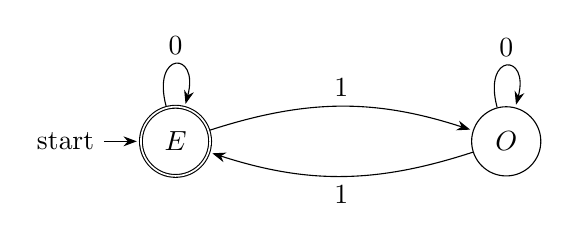
\begin{tikzpicture}[>=Stealth,shorten >=1pt,node distance=4.2cm,on grid,auto]
  \node[state,initial,accepting] (E) {$E$};
  \node[state] (O) [right=of E] {$O$};
  \path[->]
    (E) edge[loop above] node {$0$} (E)
        edge[bend left=18] node {$1$} (O)
    (O) edge[loop above] node {$0$} (O)
        edge[bend left=18] node {$1$} (E);
\end{tikzpicture}
\end{center}
Here $E$ outputs $\tau=0$ and $\eps=+1$, while $O$ outputs $\tau=1$ and
$\eps=-1$.

\begin{definition}
The $2$-kernel of a sequence $a=(a_n)_{n\ge0}$ is
\[
 \mathcal K_2(a)=\bigl\{(a_{2^en+r})_{n\ge0}:e\ge0,\ 0\le r<2^e\bigr\}.
\]
\end{definition}

\begin{proposition}[Minimal kernel]\label{prop:kernel}
The signed Thue--Morse sequence has
\[
  \mathcal K_2(\eps)=\{\eps,-\eps\},
\]
and the zero--one sequence has
\[
  \mathcal K_2(\tau)=\{\tau,1-\tau\}.
\]
Consequently both are $2$-automatic.
\end{proposition}

\begin{proof}
Iterating \cref{eq:no-carry-concat} gives
$\eps_{2^en+r}=\eps_n\eps_r$.  Since $\eps_r\in\{\pm1\}$, each kernel element
is either $\eps$ or $-\eps$, and both occur.  The zero--one statement follows
from \cref{eq:tau-eps-conversion}.
\end{proof}

\subsection{Tensor and Walsh descriptions}

Let $n=(b_{m-1}\cdots b_1b_0)_2$ with leading zeroes allowed.  Then
\begin{equation}\label{eq:tensor-character}
 \eps_n=\prod_{j=0}^{m-1}(-1)^{b_j(n)}
       =\bigotimes_{j=0}^{m-1}(1,-1)_{b_j(n)}.
\end{equation}
Hence the length-$2^m$ vector is the Kronecker power
\begin{equation}\label{eq:kronecker}
 (\eps_0,\ldots,\eps_{2^m-1})=(1,-1)^{\otimes m}.
\end{equation}
In the additive group $(\Ftwo)^m$, it is the Walsh character
\begin{equation}\label{eq:walsh-character}
  \eps_n=(-1)^{\langle \mathbf 1,\mathbf b(n)\rangle},
  \qquad \mathbf 1=(1,\ldots,1).
\end{equation}
This viewpoint makes orthogonality immediate: over the full Boolean cube,
$\eps$ is orthogonal to every Walsh character except itself.

\subsection{Overlap-free structure}

A finite or infinite word contains an \emph{overlap} if it has a factor of the
form $aXaXa$, where $a$ is a letter and $X$ is a possibly empty word.  A
classical theorem of Thue says that the fixed point of \cref{eq:morphism} is
overlap-free.  In particular it contains no cube $XXX$ with $X\ne\varnothing$.
This combinatorial fact is not visible in a single arithmetic formula, but it
is central to the sequence's original role in combinatorics on words.  It also
illustrates why a complete atlas needs both formulae and substitution
structure.

\section{Digit, floor, fractional-part, and trigonometric formulae}

\subsection{Extracting a binary digit}

For every $j\ge0$,
\begin{equation}\label{eq:binary-digit-floor}
 b_j(n)=\floor{\frac{n}{2^j}}-2\floor{\frac{n}{2^{j+1}}}
       =\floor{\frac{n}{2^j}}\bmod 2.
\end{equation}
Summing over $j$ yields several exact formulae.

\begin{theorem}[Floor and fractional-part formulae]\label{thm:floor-formulas}
For every $n\ge0$,
\begin{align}
 \bitsum(n)
 &=n-\sum_{j\ge1}\floor{\frac{n}{2^j}},\label{eq:legendre-floor}\\
 &=\sum_{j\ge1}\frac{[n]_{2^j}}{2^j},\label{eq:remainder-sum}\\
 &=\sum_{j\ge1}\fracp{\frac{n}{2^j}}.\label{eq:fractional-parts}
\end{align}
The floor sum is finite; the latter two series converge geometrically after
$2^j>n$.
\end{theorem}

\begin{proof}
Summing \cref{eq:binary-digit-floor} over $j\ge0$ telescopes:
\[
 \sum_{j\ge0}b_j(n)
 =\sum_{j\ge0}\floor{\frac n{2^j}}
  -2\sum_{j\ge0}\floor{\frac n{2^{j+1}}}
 =n-\sum_{j\ge1}\floor{\frac n{2^j}}.
\]
Since $n=2^j\floor{n/2^j}+[n]_{2^j}$ and
$\sum_{j\ge1}n/2^j=n$, substitution gives the remainder and
fractional-part forms.
\end{proof}

Consequently
\begin{equation}\label{eq:floor-sign}
  \eps_n=(-1)^{n-\sum_{j\ge1}\floor{n/2^j}}.
\end{equation}

\subsection{Products of local digit signs}

Because $1-2b_j(n)=(-1)^{b_j(n)}$,
\begin{equation}\label{eq:digit-product}
 \eps_n=\prod_{j\ge0}(1-2b_j(n)).
\end{equation}
This is finite because all sufficiently high digits vanish.  Replacing a bit by
a cosine gives
\begin{equation}\label{eq:cos-floor-product}
 \eps_n=\prod_{j\ge0}\cos\!\left(\pi\floor{\frac{n}{2^j}}\right),
\end{equation}
again with all but finitely many factors equal to $1$.  A single trigonometric
formula is
\begin{equation}\label{eq:single-cosine}
 \eps_n=\cos(\pi\bitsum(n)),
 \qquad
 \tau(n)=\sin^2\!\left(\frac{\pi}{2}\bitsum(n)\right).
\end{equation}

\subsection{A sinc sign interpolation}

Define $\sinc x=\sin x/x$ for $x\ne0$ and $\sinc 0=1$, and put
\begin{equation}\label{eq:sinc-product}
 \Phi(x)=\prod_{j=0}^{\infty}\sinc\!\left(\frac{\pi x}{2^j}\right).
\end{equation}
The product converges locally uniformly because
$1-\sinc y=\bigO(y^2)$ near $0$.

\begin{proposition}[Signs between consecutive integers]\label{prop:sinc-sign}
For every integer $N\ge0$ and every $x\in(N,N+1)$,
\begin{equation}\label{eq:sinc-sign-interval}
 \sgn\Phi(x)=\eps_N.
\end{equation}
In particular,
\begin{equation}\label{eq:sinc-half-integer}
 \eps_N=\sgn\Phi\!\left(N+\frac12\right).
\end{equation}
\end{proposition}

\begin{proof}
For positive $x$ the denominator of every sinc factor is positive.  Thus its
sign is the sign of $\sin(\pi x/2^j)$.  For fixed $x\in(N,N+1)$, the number of
negative factors equals, modulo $2$, the sum of the binary digits of $N$.
One way to see this is to compare signs recursively: from
\[
 \Phi(2x)=\sinc(2\pi x)\Phi(x)
\]
and the sign of $\sin(2\pi x)$ on half-unit intervals, the two interval signs
above $N$ are $\eps_N$ and $-\eps_N$, exactly as in
\cref{eq:signed-dyadic-recursion}.  Since the initial interval $(0,1)$ has
positive sign, induction proves the claim.
\end{proof}

\begin{remark}
The zeros of $\Phi$ at the positive integers make it a continuous analytic
carrier of a discontinuous symbolic pattern.  The formula does not interpolate
$\eps_N$ by value; it interpolates it by the sign on complementary intervals.
\end{remark}

\section{Factorial valuations, central binomials, Catalan numbers, and carries}

\subsection{Legendre's identity in base two}

\begin{theorem}[Legendre]\label{thm:legendre}
For every $n\ge0$,
\begin{equation}\label{eq:legendre}
 \vtwo(n!)=\sum_{j\ge1}\floor{\frac n{2^j}}=n-\bitsum(n).
\end{equation}
Therefore
\begin{equation}\label{eq:factorial-sign}
 \eps_n=(-1)^{n-\vtwo(n!)}=(-1)^{n+\vtwo(n!)}.
\end{equation}
\end{theorem}

\begin{proof}
Every multiple of $2$ contributes at least one factor $2$, every multiple of
$4$ contributes one additional factor, and so on.  This gives the floor sum.
The second equality is \cref{eq:legendre-floor}.
\end{proof}

\subsection{A single central binomial coefficient}

\begin{theorem}[Central-binomial valuation]\label{thm:central-binomial}
For every $n\ge0$,
\begin{equation}\label{eq:central-binomial-v2}
 \vtwo\binom{2n}{n}=\bitsum(n).
\end{equation}
Consequently
\begin{equation}\label{eq:central-binomial-thue-morse}
 \boxed{\ \eps_n=(-1)^{\vtwo\binom{2n}{n}},\qquad
 \tau(n)=\res{\vtwo\binom{2n}{n}}{2}.\ }
\end{equation}
\end{theorem}

\begin{proof}
By \cref{eq:legendre},
\[
 \vtwo\binom{2n}{n}
 =\vtwo((2n)!)-2\vtwo(n!)
 =(2n-\bitsum(2n))-2(n-\bitsum(n)).
\]
Since $\bitsum(2n)=\bitsum(n)$, this is $\bitsum(n)$.
\end{proof}

This formula is particularly economical: a statistic of all binary digits is
recovered from the $2$-adic order of one classical integer.

\subsection{Catalan numbers}

Let
\[
 \Cat_n=\frac1{n+1}\binom{2n}{n}.
\]

\begin{proposition}[Catalan valuation]\label{prop:catalan}
For $n\ge0$,
\begin{equation}\label{eq:catalan-v2}
 \vtwo(\Cat_n)=\bitsum(n+1)-1.
\end{equation}
Hence for $n\ge0$,
\begin{equation}\label{eq:catalan-thue-morse}
 \eps_{n+1}=-(-1)^{\vtwo(\Cat_n)},
 \qquad
 \tau(n+1)=1-\res{\vtwo(\Cat_n)}{2}.
\end{equation}
\end{proposition}

\begin{proof}
By \cref{thm:central-binomial},
$\vtwo(\Cat_n)=\bitsum(n)-\vtwo(n+1)$.  If $r=\vtwo(n+1)$, then adding $1$ to
$n$ replaces exactly $r$ trailing $1$'s by $0$'s and then changes one $0$ to
$1$.  Thus $\bitsum(n+1)=\bitsum(n)-r+1$.
\end{proof}

\subsection{Kummer's theorem and the carry-corrected addition law}

\begin{theorem}[Kummer in base two]\label{thm:kummer}
The number of carries produced when adding $a$ and $b$ in base two is
\begin{equation}\label{eq:kummer}
 c_2(a,b)=\vtwo\binom{a+b}{a}
         =\bitsum(a)+\bitsum(b)-\bitsum(a+b).
\end{equation}
\end{theorem}

\begin{proof}
The valuation identity follows from \cref{eq:legendre}:
\begin{align*}
 \vtwo\binom{a+b}{a}
 &=a+b-\bitsum(a+b)-(a-\bitsum(a))-(b-\bitsum(b))\\
 &=\bitsum(a)+\bitsum(b)-\bitsum(a+b).
\end{align*}
Each binary carry reduces the total digit sum by exactly one relative to the
no-carry sum, counted with propagation; this gives the carry interpretation.
\end{proof}

\begin{theorem}[Carry-corrected multiplicativity]\label{thm:carry-law}
For all $a,b\ge0$,
\begin{equation}\label{eq:carry-law}
 \boxed{\ \eps_{a+b}=\eps_a\eps_b
     (-1)^{\vtwo\binom{a+b}{a}}.\ }
\end{equation}
Equivalently,
\begin{equation}\label{eq:tau-carry-law}
 \tau(a+b)\equiv \tau(a)+\tau(b)+\vtwo\binom{a+b}{a}\pmod2.
\end{equation}
\end{theorem}

\begin{proof}
Reduce \cref{eq:kummer} modulo $2$ and exponentiate $-1$.
\end{proof}

\begin{example}
Take $a=13=(1101)_2$ and $b=7=(0111)_2$.  Then
$\bitsum(a)=3$, $\bitsum(b)=3$, $a+b=20=(10100)_2$, and
$\bitsum(a+b)=2$.  Hence $\vtwo\binom{20}{13}=4$ and
$\eps_{20}=\eps_{13}\eps_7(-1)^4=( -1)(-1)=+1$, as expected.
\end{example}

\subsection{Subtraction and borrow counts}

For $0\le b\le a$, Kummer also gives
\begin{equation}\label{eq:borrow-law}
 \vtwo\binom ab=\bitsum(b)+\bitsum(a-b)-\bitsum(a),
\end{equation}
which counts borrows in the subtraction $a-b$.  Thus
\begin{equation}\label{eq:subtraction-thue-morse}
 \eps_{a-b}=\eps_a\eps_b(-1)^{\vtwo\binom ab}.
\end{equation}
This is the subtraction analogue of \cref{eq:carry-law}.

\section{Pascal's triangle, Lucas support, and log-free row formulae}

\subsection{Odd entries and the Boolean submask lattice}

For nonnegative integers $k,n$, write $k\submask n$ when every $1$-bit of
$k$ occurs in a position where $n$ also has a $1$-bit.  Equivalently,
$k\mathbin{\&}\neg n=0$.

\begin{theorem}[Lucas in base two]\label{thm:lucas}
For $0\le k\le n$,
\begin{equation}\label{eq:lucas-submask}
 \binom nk\equiv1\pmod2
 \quad\Longleftrightarrow\quad
 k\submask n.
\end{equation}
Consequently the number of odd entries in row $n$ of Pascal's triangle is
\begin{equation}\label{eq:glaisher}
 \mathcal O(n):=\#\left\{0\le k\le n:\binom nk\text{ is odd}\right\}
 =2^{\bitsum(n)}.
\end{equation}
\end{theorem}

\begin{proof}
Lucas's congruence writes
\[
 \binom nk\equiv\prod_{j\ge0}\binom{b_j(n)}{b_j(k)}\pmod2.
\]
A factor vanishes precisely when $b_j(k)=1$ and $b_j(n)=0$.  Therefore odd
entries are indexed by subsets of the $\bitsum(n)$ occupied bit positions,
giving $2^{\bitsum(n)}$ choices.
\end{proof}

The support set
\begin{equation}\label{eq:pascal-support}
 \mathcal B(n)=\{k:k\submask n\}
\end{equation}
is a Boolean lattice of rank $\bitsum(n)$.  Its Möbius function from $0$ to
$k$ is
\begin{equation}\label{eq:boolean-mobius}
 \mu_{\mathcal B(n)}(0,k)=(-1)^{\bitsum(k)}=\eps_k.
\end{equation}
Thus the signed Thue--Morse value is literally the Möbius sign of the binary
submask lattice.

\subsection{The binomial--logarithm formula and its exact variants}

Taking a base-two logarithm in \cref{eq:glaisher} gives
\begin{equation}\label{eq:binomial-log}
 \bitsum(n)=\log_2\mathcal O(n),
 \qquad
 \tau(n)=\res{\log_2\mathcal O(n)}{2},
 \qquad
 \eps_n=(-1)^{\log_2\mathcal O(n)}.
\end{equation}
This is exact because $\mathcal O(n)$ is a power of two.  The odd-count itself
can be written without a parity predicate:
\begin{align}
 \mathcal O(n)
 &=\sum_{k=0}^n \frac{1-(-1)^{\binom nk}}2,\label{eq:odd-count-sign}\\
 &=\sum_{k=0}^n\sin^2\!\left(\frac\pi2\binom nk\right),\label{eq:odd-count-trig}\\
 &=\frac12\left(n+1-\sum_{k=0}^n\cos\!\left(\pi\binom nk\right)\right).
 \label{eq:odd-count-cos}
\end{align}
These forms explain the binomial--logarithm identity in the companion
Fabius-function exposition.

\subsection{A log-free formula modulo three}

Let $[a]_q\in\{0,1,\ldots,q-1\}$ denote the least nonnegative residue of the
integer $a$ modulo $q$.  Since $2^r\equiv1$ or $2\pmod3$ according as $r$ is
even or odd, \cref{eq:glaisher} immediately removes the logarithm.

\begin{theorem}[Log-free Pascal formula]\label{thm:log-free-pascal}
For every $n\ge0$,
\begin{equation}\label{eq:log-free-pascal}
 \boxed{\quad
 \tau(n)=[\mathcal O(n)]_3-1,
 \qquad
 \eps_n=3-2[\mathcal O(n)]_3.
 \quad}
\end{equation}
Here $[\mathcal O(n)]_3$ is always $1$ or $2$, never $0$.
\end{theorem}

\begin{proof}
By \cref{eq:glaisher},
$[\mathcal O(n)]_3=[2^{\bitsum(n)}]_3$.  This residue equals $1$ when
$\bitsum(n)$ is even and $2$ when it is odd.
\end{proof}

There is also a formula involving a single signed row statistic.  Define
\begin{equation}\label{eq:signed-row-statistic}
 \Sigma(n)=\sum_{k=1}^{n}(-1)^{\binom nk},
\end{equation}
with the empty sum $\Sigma(0)=0$.

\begin{proposition}[Signed-row residue]\label{prop:signed-row-residue}
For every $n\ge0$,
\begin{equation}\label{eq:signed-row-residue}
 \boxed{\qquad \tau(n)=[2n+\Sigma(n)]_3.\qquad}
\end{equation}
Equivalently,
\begin{equation}\label{eq:signed-row-trig}
 \tau(n)=\left[2n+\sum_{k=1}^{n}
          \cos\!\left(\pi\binom nk\right)\right]_3.
\end{equation}
\end{proposition}

\begin{proof}
Among $k=1,\ldots,n$, exactly $\mathcal O(n)-1$ binomial coefficients are odd.
Therefore
\[
 \Sigma(n)=\bigl(n-\mathcal O(n)+1\bigr)-\bigl(\mathcal O(n)-1\bigr)
          =n+2-2\mathcal O(n).
\]
Hence $2n+\Sigma(n)\equiv2-2\mathcal O(n)\pmod3$, which is $0$ when
$\mathcal O(n)\equiv1$ and $1$ when $\mathcal O(n)\equiv2$.
\end{proof}

\subsection{A one-parameter row statistic}

For an indeterminate or complex parameter $u$, define
\begin{equation}\label{eq:Ru-definition}
 R_u(n)=\sum_{k=0}^{n}u^{\binom nk\bmod2}.
\end{equation}

\begin{identity}[Pascal row partition function]\label{id:Ru}
\begin{equation}\label{eq:Ru}
 R_u(n)=n+1+(u-1)2^{\bitsum(n)}.
\end{equation}
\end{identity}

\begin{proof}
Every even entry contributes $1$, and every odd entry contributes $u$.
There are $2^{\bitsum(n)}$ odd entries.
\end{proof}

Specializations organize several earlier formulae:
\begin{align*}
 R_0(n)&=n+1-2^{\bitsum(n)} &&\text{counts even entries},\\
 R_1(n)&=n+1,\\
 R_{-1}(n)&=n+1-2^{\bitsum(n)+1}
           =\sum_{k=0}^{n}(-1)^{\binom nk},\\
 \left.\frac{\partial}{\partial u}R_u(n)\right|_{u=1}
 &=2^{\bitsum(n)} &&\text{counts odd entries}.
\end{align*}
The parameter $u$ is therefore a compact generating device for all statistics
that distinguish only the parity of each Pascal entry.

\subsection{Nested binomial parity probes}

Lucas's theorem supplies a universal probe for binary digits of any integer
$M\ge0$:
\begin{equation}\label{eq:nested-bit-probe}
 b_r(M)\equiv\binom{M}{2^r}\pmod2.
\end{equation}
Taking $M=\binom nk$ yields nested binomial coefficients
\begin{equation}\label{eq:nested-pascal-probe}
 b_r\!\left(\binom nk\right)
 \equiv
 \binom{\binom nk}{2^r}\pmod2.
\end{equation}
Thus every binary digit of every Pascal entry can be represented by the parity
of another binomial coefficient.  Summing over $r$ gives an exact, though not
usually economical, formula
\begin{equation}\label{eq:nested-digit-sum}
 \bitsum\!\left(\binom nk\right)
 =\sum_{r\ge0}
   \left[\binom{\binom nk}{2^r}\right]_2.
\end{equation}
This hierarchy is useful when a formal library already has Lucas congruences
but not bit-extraction lemmas for arbitrary integers.

\subsection{Power-of-two rows and cyclotomic sparsity}

For $m\ge0$, all interior coefficients of $(1+x)^{2^m}$ are even, so over
$\Ftwo$
\begin{equation}\label{eq:freshman-dream}
 (1+x)^{2^m}=1+x^{2^m}.
\end{equation}
More generally, if $n=\sum_{j\in J(n)}2^j$, then
\begin{equation}\label{eq:lucas-polynomial}
 (1+x)^n
 \equiv\prod_{j\in J(n)}(1+x^{2^j})
 \pmod2.
\end{equation}
The coefficient support on the right is exactly the submask set
$\mathcal B(n)$.  This polynomial form of Lucas's theorem will reappear in the
sparse Prouhet identities of \cref{sec:sparse-prouhet}.

\section{Multinomial parity and higher-dimensional support}

\subsection{Odd multinomial coefficients}

For $r\ge2$ and $n_1+\cdots+n_r=n$, write
\[
 \binom{n}{n_1,\ldots,n_r}=\frac{n!}{n_1!\cdots n_r!}.
\]

\begin{theorem}[Odd multinomial support]\label{thm:odd-multinomial}
The number of odd multinomial coefficients in the full $r$-nomial layer of
weight $n$ is
\begin{equation}\label{eq:odd-multinomial-count}
 \mathcal O_r(n)
 :=\#\left\{(n_1,\ldots,n_r):\sum n_i=n,
       \binom{n}{n_1,\ldots,n_r}\text{ odd}\right\}
 =r^{\bitsum(n)}.
\end{equation}
More precisely, the parity-support polynomial is
\begin{equation}\label{eq:multinomial-support-polynomial}
 \sum_{\substack{n_1+\cdots+n_r=n\\
       \binom{n}{n_1,\ldots,n_r}\text{ odd}}}
 x_1^{n_1}\cdots x_r^{n_r}
 =\prod_{j\in J(n)}
   \left(x_1^{2^j}+\cdots+x_r^{2^j}\right).
\end{equation}
\end{theorem}

\begin{proof}
In characteristic two,
\[
 (x_1+\cdots+x_r)^n
 =\prod_{j\in J(n)}(x_1+\cdots+x_r)^{2^j}
 =\prod_{j\in J(n)}(x_1^{2^j}+\cdots+x_r^{2^j}).
\]
Every occupied binary position of $n$ must be assigned independently to one of
the $r$ components.  There are $r^{\bitsum(n)}$ assignments, and no carries
are permitted among the component digit sums.
\end{proof}

\begin{corollary}[Multinomial recovery of Thue--Morse]\label{cor:multinomial-recovery}
For any fixed integer $r\ge2$,
\begin{equation}\label{eq:multinomial-log-recovery}
 \tau(n)=\left[\log_r\mathcal O_r(n)\right]_2,
 \qquad
 \eps_n=(-1)^{\log_r\mathcal O_r(n)}.
\end{equation}
When $r\equiv-1\pmod3$, the logarithm can again be removed:
\begin{equation}\label{eq:multinomial-logfree}
 \tau(n)=[\mathcal O_r(n)]_3-1,
 \qquad
 \eps_n=3-2[\mathcal O_r(n)]_3.
\end{equation}
\end{corollary}

\begin{proof}
The logarithmic formula is immediate from \cref{eq:odd-multinomial-count}.  If
$r\equiv2\pmod3$, then $r^{\bitsum(n)}$ alternates between residues $1$ and
$2$ according to the parity of $\bitsum(n)$.
\end{proof}

\subsection{Valuation and carry interpretation}

Legendre's identity gives
\begin{equation}\label{eq:multinomial-v2}
 \vtwo\binom{n}{n_1,\ldots,n_r}
 =\sum_{i=1}^r\bitsum(n_i)-\bitsum(n).
\end{equation}
This is zero precisely when adding the $n_i$ in base two produces no carry.
Thus \cref{thm:odd-multinomial} is a carry-free allocation theorem: each
occupied bit of $n$ chooses exactly one component.

\subsection{A multivariate Boolean lattice}

The support in \cref{eq:multinomial-support-polynomial} is the Cartesian
product of $\bitsum(n)$ copies of an $r$-element choice set.  For $r=2$ it is
the Boolean submask lattice.  For general $r$ it is the discrete cube
$\{1,\ldots,r\}^{\bitsum(n)}$.  This makes the exponent
$r^{\bitsum(n)}$ conceptually inevitable and suggests higher-dimensional
Walsh transforms adapted to multinomial support.

\section{Evil and odious numbers, counting, and exact summatory formulae}

An integer is called \emph{evil} when $\tau(n)=0$ and \emph{odious} when
$\tau(n)=1$.  Let $E_j$ and $O_j$ be the $j$th evil and odious nonnegative
integers, indexed from $j=0$.

\begin{theorem}[Exact enumerators]\label{thm:evil-odious-enumerators}
For every $j\ge0$,
\begin{equation}\label{eq:evil-odious-enumerators}
 \boxed{\quad E_j=2j+\tau(j),\qquad
 O_j=2j+1-\tau(j).\quad}
\end{equation}
In particular,
\begin{equation}\label{eq:evil-odious-gap}
 O_j-E_j=1-2\tau(j)=\eps_j.
\end{equation}
\end{theorem}

\begin{proof}
The pair $(2j,2j+1)$ has signs $(\eps_j,-\eps_j)$ by
\cref{eq:signed-dyadic-recursion}.  Therefore exactly one member of the pair is
evil and one is odious.  If $\tau(j)=0$, they occur in the order
$(E_j,O_j)=(2j,2j+1)$; if $\tau(j)=1$, the order is reversed.
\end{proof}

\subsection{Exact prefix sums}

Define the signed prefix sum
\begin{equation}\label{eq:prefix-sum-def}
 S(N)=\sum_{n=0}^{N-1}\eps_n,
 \qquad S(0)=0.
\end{equation}

\begin{theorem}[Exact prefix discrepancy]\label{thm:prefix-discrepancy}
For every $q\ge0$,
\begin{equation}\label{eq:prefix-discrepancy}
 S(2q)=0,
 \qquad
 S(2q+1)=\eps_q.
\end{equation}
Hence $S(N)\in\{-1,0,1\}$ for every $N$.
\end{theorem}

\begin{proof}
Pair consecutive terms:
$\eps_{2j}+\eps_{2j+1}=\eps_j-\eps_j=0$.  An odd prefix has the additional
term $\eps_{2q}=\eps_q$.
\end{proof}

Let
\[
 E(N)=\#\{0\le n<N:\tau(n)=0\},
 \qquad
 O(N)=\#\{0\le n<N:\tau(n)=1\}.
\]
Then
\begin{equation}\label{eq:evil-odious-counts}
 E(N)=\frac{N+S(N)}2,
 \qquad
 O(N)=\frac{N-S(N)}2.
\end{equation}
Thus every prefix has exactly balanced evil and odious counts when $N$ is
even, and imbalance one when $N$ is odd.

\subsection{Interval discrepancy}

For integers $A,B\ge0$, put
\[
 D(A,B)=S(B)-S(A).
\]
When $A<B$, this is the signed interval sum
$D(A,B)=\sum_{n=A}^{B-1}\eps_n$.

\begin{corollary}[Uniform interval bound]\label{cor:interval-discrepancy}
For all integers $0\le A<B$,
\begin{equation}\label{eq:interval-discrepancy}
 |D(A,B)|\le2.
\end{equation}
More precisely, for $a,b\ge0$,
\begin{align}
 D(2a,2b)&=0,\label{eq:interval-even-even}\\
 D(2a,2b+1)&=\eps_b,\label{eq:interval-even-odd}\\
 D(2a+1,2b)&=-\eps_a,\label{eq:interval-odd-even}\\
 D(2a+1,2b+1)&=\eps_b-\eps_a.\label{eq:interval-odd-odd}
\end{align}
Thus opposite-parity endpoints give $|D(A,B)|=1$; even endpoints give zero;
and odd endpoints give one of $-2,0,2$.
\end{corollary}

\begin{proof}
Substitute the exact prefix values
$S(2q)=0$ and $S(2q+1)=\eps_q$ into $D(A,B)=S(B)-S(A)$.
\end{proof}

\begin{remark}
This exact discrepancy bound is special to unweighted sums.  Exponential sums
$\sum_{n<N}\eps_n\e^{2\pi\ii n\alpha}$ have much subtler growth; the sharp
uniform exponent is discussed in \cref{sec:gelfond}.
\end{remark}

\section{Finite generating products and their algebra}

\subsection{The coefficient product}

\begin{theorem}[Finite product identity]\label{thm:finite-product}
For every $m\ge0$,
\begin{equation}\label{eq:finite-product}
 \boxed{\quad
 P_m(z):=\sum_{n=0}^{2^m-1}\eps_nz^n
 =\prod_{j=0}^{m-1}(1-z^{2^j}).
 \quad}
\end{equation}
\end{theorem}

\begin{proof}
Expanding the product means choosing either $1$ or $-z^{2^j}$ from each
factor.  A choice set $J\subseteq\{0,\ldots,m-1\}$ contributes
$(-1)^{|J|}z^{\sum_{j\in J}2^j}$.  Every exponent $0\le n<2^m$ has a unique
binary choice set, and the sign is $(-1)^{\bitsum(n)}$.
\end{proof}

The product obeys two complementary recursions:
\begin{align}
 P_{m+1}(z)&=(1-z^{2^m})P_m(z),\label{eq:P-adjoin}\\
 P_m(z)&=(1-z)P_{m-1}(z^2)\qquad(m\ge1).\label{eq:P-mahler-finite}
\end{align}
The first appends the highest bit; the second separates the least significant
bit.

\subsection{Reciprocity and cyclotomic factorization}

Let $D_m=2^m-1=\deg P_m$.  Then
\begin{equation}\label{eq:P-reciprocity}
 z^{D_m}P_m(z^{-1})=(-1)^mP_m(z).
\end{equation}
Equating coefficients gives the reflection rule
\begin{equation}\label{eq:reflection-rule}
 \eps_{D_m-n}=(-1)^m\eps_n,
 \qquad 0\le n\le D_m.
\end{equation}
This is the complement-all-bits symmetry of an $m$-bit word.

Factoring each $1-z^{2^j}$ into dyadic cyclotomic factors gives
\begin{equation}\label{eq:cyclotomic-factorization}
 P_m(z)=(1-z)^m
 \prod_{r=0}^{m-2}(1+z^{2^r})^{m-1-r}.
\end{equation}
Therefore the complete zero set consists of roots of unity of order a power of
two.  The multiplicity of a primitive $2^{r+1}$st root is $m-1-r$, while
$z=1$ has multiplicity $m$.

\subsection{Coefficient extraction and binary uniqueness}

The finite product yields several exact coefficient formulae:
\begin{align}
 \eps_n
 &=\coeff n{\prod_{j\ge0}(1-z^{2^j})},\label{eq:coefficient-infinite-formal}\\
 \eps_n
 &=\sum_{J\subseteq\{0,\ldots,m-1\}}
    (-1)^{|J|}\ind\!\left(n=\sum_{j\in J}2^j\right)
    \quad(0\le n<2^m),\label{eq:subset-coefficient}\\
 \tau(n)&=\frac12\left(1-\coeff n{P_m(z)}\right)
    \qquad(0\le n<2^m).
\end{align}
The sum in \cref{eq:subset-coefficient} has exactly one nonzero term.  Its
importance is structural rather than computational: it realizes Thue--Morse as
the signed incidence function of binary subset sums.

\subsection{Weighted digit sums}

A useful umbrella product is
\begin{equation}\label{eq:Fu}
 F_u(z)=\sum_{n\ge0}u^{\bitsum(n)}z^n
       =\prod_{j\ge0}(1+u z^{2^j}),
 \qquad |z|<1.
\end{equation}
It satisfies
\begin{equation}\label{eq:Fu-mahler}
 F_u(z)=(1+uz)F_u(z^2).
\end{equation}
The cases $u=1$ and $u=-1$ are
\begin{equation}\label{eq:Fu-special}
 F_1(z)=\frac1{1-z},
 \qquad
 F_{-1}(z)=E(z).
\end{equation}
Differentiating with respect to $u$ at $u=1$ gives the ordinary generating
function for the binary digit sum:
\begin{equation}\label{eq:digit-sum-ogf}
 \sum_{n\ge0}\bitsum(n)z^n
 =\frac1{1-z}\sum_{j\ge0}\frac{z^{2^j}}{1+z^{2^j}}.
\end{equation}
Higher $u$-derivatives generate the falling-factorial moments
$\fall{\bitsum(n)}r$.

\section{Infinite products, Mahler equations, and coefficient recurrences}

\subsection{The signed analytic generating function}

For $|z|<1$, the finite products converge locally uniformly to
\begin{equation}\label{eq:E-product}
 E(z)=\sum_{n\ge0}\eps_nz^n
     =\prod_{j=0}^{\infty}(1-z^{2^j}).
\end{equation}
The first factor separates:
\begin{equation}\label{eq:E-mahler}
 \boxed{\qquad E(z)=(1-z)E(z^2),\qquad E(0)=1.\qquad}
\end{equation}
Iterating $r$ times gives the lacunary quotient
\begin{equation}\label{eq:lacunary-quotient}
 \frac{E(z)}{E(z^{2^r})}=\prod_{j=0}^{r-1}(1-z^{2^j})=P_r(z).
\end{equation}
As $r\to\infty$, $E(z^{2^r})\to1$, recovering the infinite product.

\subsection{The zero--one generating function}

Using \cref{eq:tau-eps-conversion},
\begin{equation}\label{eq:T-from-E}
 \boxed{\qquad
 T(z)=\sum_{n\ge0}\tau(n)z^n
 =\frac1{2(1-z)}-\frac12E(z).
 \qquad}
\end{equation}
Separating even and odd indices gives the inhomogeneous Mahler equation
\begin{equation}\label{eq:T-mahler}
 \boxed{\qquad
 T(z)=(1-z)T(z^2)+\frac{z}{1-z^2}.
 \qquad}
\end{equation}
Indeed,
\begin{align*}
 T(z)
 &=\sum_{n\ge0}\tau(2n)z^{2n}
   +\sum_{n\ge0}\tau(2n+1)z^{2n+1}\\
 &=T(z^2)+z\left(\frac1{1-z^2}-T(z^2)\right).
\end{align*}

\subsection{Logarithmic derivative and the ruler function}

Taking a logarithm in \cref{eq:E-product},
\begin{align}
 \log E(z)
 &=\sum_{j\ge0}\log(1-z^{2^j})\notag\\
 &=-\sum_{j\ge0}\sum_{q\ge1}\frac{z^{q2^j}}q
 =-\sum_{r\ge1}\frac{a_r}{r}z^r,\label{eq:log-E}
\end{align}
where
\begin{equation}\label{eq:ruler-coeff}
 a_r=\sum_{2^j\mid r}2^j=2^{\vtwo(r)+1}-1.
\end{equation}
Thus
\begin{equation}\label{eq:log-derivative-E}
 \frac{zE'(z)}{E(z)}=-\sum_{r\ge1}a_rz^r.
\end{equation}
The coefficient $a_r$ is an affine function of the ruler sequence
$2^{\vtwo(r)}$.

\begin{theorem}[Convolution recurrence]\label{thm:convolution-recurrence}
With $\eps_0=1$, the signed Thue--Morse coefficients satisfy
\begin{equation}\label{eq:convolution-recurrence}
 \boxed{\qquad
 n\eps_n=-\sum_{r=1}^{n}
       \bigl(2^{\vtwo(r)+1}-1\bigr)\eps_{n-r}
 \qquad(n\ge1).}
\end{equation}
\end{theorem}

\begin{proof}
Multiply \cref{eq:log-derivative-E} by $E(z)$ and compare the coefficient of
$z^n$.
\end{proof}

This recurrence is arithmetically very different from the dyadic recursion:
it computes $\eps_n$ from all preceding values, weighted by a valuation
sequence.

\subsection{Bell-polynomial formula}

Let $\Bell_n(x_1,\ldots,x_n)$ be the complete exponential Bell polynomial,
defined by
\begin{equation}\label{eq:Bell-definition}
 \exp\!\left(\sum_{r\ge1}x_r\frac{z^r}{r!}\right)
 =\sum_{n\ge0}\Bell_n(x_1,\ldots,x_n)\frac{z^n}{n!}.
\end{equation}
Set
\begin{equation}\label{eq:Bell-xr}
 x_r=-(r-1)!\bigl(2^{\vtwo(r)+1}-1\bigr).
\end{equation}
Then \cref{eq:log-E} gives the exact formula
\begin{equation}\label{eq:Bell-epsilon}
 \boxed{\qquad
 \eps_n=\frac1{n!}\Bell_n(x_1,\ldots,x_n).
 \qquad}
\end{equation}
This is useful when a symbolic algebra system has native Bell-polynomial
support.

\subsection{A determinant formula}

For $n\ge1$, define the lower-Hessenberg matrix
\begin{equation}\label{eq:Hn}
 H_n=\begin{pmatrix}
 a_1&1&0&0&\cdots&0\\
 a_2&a_1&2&0&\cdots&0\\
 a_3&a_2&a_1&3&\ddots&\vdots\\
 \vdots&\vdots&\ddots&\ddots&\ddots&0\\
 a_{n-1}&a_{n-2}&\cdots&a_2&a_1&n-1\\
 a_n&a_{n-1}&\cdots&a_3&a_2&a_1
 \end{pmatrix},
 \qquad a_r=2^{\vtwo(r)+1}-1.
\end{equation}

\begin{theorem}[Hessenberg determinant]\label{thm:Hessenberg}
For every $n\ge1$,
\begin{equation}\label{eq:Hessenberg-epsilon}
 \boxed{\qquad
 \eps_n=\frac{(-1)^n}{n!}\det H_n.
 \qquad}
\end{equation}
In particular,
\begin{equation}\label{eq:Hessenberg-factorial}
 |\det H_n|=n!.
\end{equation}
\end{theorem}

\begin{proof}
Expansion of a lower-Hessenberg determinant along the last row gives exactly
the coefficient recurrence associated with
$E(z)=\exp(-\sum_{r\ge1}a_rz^r/r)$.  Equivalently, this is the standard
determinantal form of complete Bell polynomials applied to
\cref{eq:Bell-epsilon}.  The absolute-value statement follows from
$\eps_n\in\{\pm1\}$.
\end{proof}

\subsection{Euler-transform form}

The product \cref{eq:E-product} is also an Euler transform with exponents
supported at powers of two:
\begin{equation}\label{eq:euler-transform}
 E(z)=\prod_{r\ge1}(1-z^r)^{c_r},
 \qquad
 c_r=\begin{cases}1,&r\text{ is a power of }2,\\0,&\text{otherwise.}\end{cases}
\end{equation}
The logarithmic derivative of a general Euler product is a divisor sum.  Here
that divisor sum collapses to \cref{eq:ruler-coeff}.  This explains why the
ruler function is the natural convolution partner of Thue--Morse.

\section{Algebraic avatars in characteristic two and over the integers}

\subsection{The Artin--Schreier equation}

Reduce the coefficients of $T(z)$ modulo $2$ and regard
\[
 \Theta(z)=\sum_{n\ge0}\tau(n)z^n\in\Ftwo[[z]].
\]
Since $\Theta(z^2)=\Theta(z)^2$ in characteristic two, reducing
\cref{eq:T-mahler} gives
\begin{equation}\label{eq:theta-mod2-mahler}
 \Theta(z)=(1+z)\Theta(z)^2+\frac{z}{1+z^2}.
\end{equation}
After clearing denominators,
\begin{equation}\label{eq:theta-algebraic}
 \boxed{\quad
 (1+z)^3\Theta(z)^2+(1+z)^2\Theta(z)+z=0.
 \quad}
\end{equation}
If
\begin{equation}\label{eq:Y-definition}
 Y(z)=(1+z)\Theta(z),
\end{equation}
then \cref{eq:theta-algebraic} becomes the Artin--Schreier equation
\begin{equation}\label{eq:Artin-Schreier}
 \boxed{\qquad Y(z)^2+Y(z)=\frac{z}{1+z}.\qquad}
\end{equation}
Thus the ordinary generating series of the zero--one sequence is algebraic of
degree two over $\Ftwo(z)$.

\begin{remark}
Christol's theorem says that, over a finite field of characteristic $p$, a
coefficient sequence is $p$-automatic if and only if its generating series is
algebraic over the corresponding rational function field.  Here $p=2$, and
both directions are visible directly: the two-state automaton gives the
recursion, while the recursion gives the explicit quadratic equation.
\end{remark}

\subsection{An integer algebraic lift}

Define integers $A_n$ by $A_0=0$, $A_1=1$, and for $n\ge2$,
\begin{equation}\label{eq:integer-lift-recurrence}
 nA_n=(5-2n)A_{n-1}+3(n-1)A_{n-2}+1.
\end{equation}
Their generating function is
\begin{equation}\label{eq:integer-lift-generating}
 A(z)=\sum_{n\ge0}A_nz^n
 =\frac1{2(1-z)}
  \left(\sqrt{\frac{1+3z}{1-z}}-1\right).
\end{equation}
It satisfies
\begin{equation}\label{eq:integer-lift-algebraic}
 \boxed{\qquad
 (1-z)^3A(z)^2+(1-z)^2A(z)=z.
 \qquad}
\end{equation}

\begin{proposition}[Parity lift]\label{prop:integer-lift-parity}
For every $n\ge0$,
\begin{equation}\label{eq:integer-lift-parity}
 A_n\equiv\tau(n)\pmod2.
\end{equation}
\end{proposition}

\begin{proof}
Reducing \cref{eq:integer-lift-algebraic} modulo $2$ changes $1-z$ to $1+z$
and gives exactly \cref{eq:theta-algebraic}.  Both formal solutions have
constant term zero.  The coefficient of the first unknown term appears
linearly with unit coefficient, so the solution in $\Ftwo[[z]]$ is unique.
Therefore $A(z)\equiv\Theta(z)\pmod2$ coefficientwise.
\end{proof}

\begin{remark}
The lift is not a new definition of Thue--Morse; it is an integer sequence whose
parity shadow is Thue--Morse.  Its value lies in transferring questions about
automatic parity to an algebraic generating function over characteristic zero.
The square-root singularity also makes asymptotic tools available for $A_n$.
\end{remark}

\section{Prouhet cancellation, finite differences, and exact cubature}

\subsection{The Prouhet partition}

For $m\ge1$, partition $\{0,1,\ldots,2^m-1\}$ into
\begin{equation}\label{eq:prouhet-partition}
 \mathcal E_m=\{n<2^m:\eps_n=1\},
 \qquad
 \mathcal O_m=\{n<2^m:\eps_n=-1\}.
\end{equation}
The finite product has a zero of order $m$ at $z=1$:
\begin{equation}\label{eq:P-zero-order}
 P_m(z)=(1-z)^m
 \prod_{r=0}^{m-2}(1+z^{2^r})^{m-1-r}.
\end{equation}
This is the algebraic source of Prouhet's equal-sums phenomenon.

\begin{theorem}[Prouhet cancellation]\label{thm:prouhet}
For every integer $r$ with $0\le r<m$,
\begin{equation}\label{eq:prouhet-moments}
 \sum_{n=0}^{2^m-1}\eps_n n^r=0.
\end{equation}
Equivalently,
\begin{equation}\label{eq:prouhet-equal-powers}
 \sum_{n\in\mathcal E_m}n^r
 =\sum_{n\in\mathcal O_m}n^r
 \qquad(0\le r<m).
\end{equation}
The first nonzero moment is
\begin{equation}\label{eq:first-nonzero-moment}
 \sum_{n=0}^{2^m-1}\eps_n n^m
 =(-1)^m m!\,2^{\binom m2}.
\end{equation}
\end{theorem}

\begin{proof}
Apply the operator $(z\frac{\dd}{\dd z})^r$ to
$P_m(z)=\sum\eps_nz^n$ and evaluate at $z=1$.  The zero of order $m$ forces
vanishing for $r<m$.  For $r=m$, only the leading term of
$P_m(z)$ at $z=1$ matters:
\[
 P_m(z)=(-1)^m2^{0+1+\cdots+(m-1)}(z-1)^m+\bigO((z-1)^{m+1}).
\]
The operator $(z\dd/\dd z)^m$ has leading part $\dd^m/\dd z^m$ at $z=1$,
giving \cref{eq:first-nonzero-moment}.
\end{proof}

\subsection{The finite-difference identity}

For $h\in\R$, let
\begin{equation}\label{eq:finite-difference-def}
 \Delta_hf(x)=f(x+h)-f(x).
\end{equation}

\begin{theorem}[Thue--Morse as an iterated difference]\label{thm:finite-difference}
For every function $f$ on which the expressions are defined,
\begin{equation}\label{eq:finite-difference}
 \boxed{\qquad
 \sum_{n=0}^{2^m-1}\eps_nf(x+n)
 =(-1)^m\Delta_1\Delta_2\cdots\Delta_{2^{m-1}}f(x).
 \qquad}
\end{equation}
\end{theorem}

\begin{proof}
Let $T_hf(x)=f(x+h)$.  Then
\[
 \sum_{n<2^m}\eps_nT_n
 =\prod_{j=0}^{m-1}(I-T_{2^j})
 =(-1)^m\prod_{j=0}^{m-1}\Delta_{2^j}.
\]
Apply both sides to $f$ at $x$.
\end{proof}

Prouhet cancellation follows immediately because each finite difference lowers
the degree of a polynomial by one.

\subsection{Exact integral cubature}

If $f$ is $m$ times continuously differentiable, then
\begin{equation}\label{eq:one-difference-integral}
 \Delta_hf(x)=h\int_0^1f'(x+hu)\dd u.
\end{equation}
Iterating gives an exact integral representation.

\begin{theorem}[Cubature identity]\label{thm:cubature}
For $f\in C^m$,
\begin{equation}\label{eq:cubature}
 \boxed{\quad
 \sum_{n=0}^{2^m-1}\eps_nf(x+n)
 =(-1)^m2^{\binom m2}
  \int_{[0,1]^m}
  f^{(m)}\!\left(x+\sum_{j=0}^{m-1}2^ju_j\right)
  \dd\mathbf u.
 \quad}
\end{equation}
\end{theorem}

\begin{proof}
Apply \cref{eq:one-difference-integral} successively to
\cref{eq:finite-difference}; the product of the step sizes is
$\prod_{j=0}^{m-1}2^j=2^{\binom m2}$.
\end{proof}

\begin{corollary}[Mean-value form]\label{cor:mean-value}
If $f\in C^m$ on $[x,x+2^m-1]$, there exists
$\xi\in[x,x+2^m-1]$ such that
\begin{equation}\label{eq:mean-value}
 \sum_{n=0}^{2^m-1}\eps_nf(x+n)
 =(-1)^m2^{\binom m2}f^{(m)}(\xi).
\end{equation}
\end{corollary}

The cubature formula is stronger than a vanishing-moment statement: it
identifies the complete remainder for arbitrary smooth $f$.

\subsection{All power moments}

Define
\begin{equation}\label{eq:moment-def}
 M_{m,r}=\sum_{n=0}^{2^m-1}\eps_nn^r.
\end{equation}
The exponential generating function in $r$ is
\begin{equation}\label{eq:moment-egf}
 \sum_{r\ge0}M_{m,r}\frac{t^r}{r!}
 =P_m(\e^t)
 =\prod_{j=0}^{m-1}(1-\e^{2^jt}).
\end{equation}
Put
\[
 \varphi(x)=\frac{\e^x-1}{x}=\sum_{q\ge0}\frac{x^q}{(q+1)!}.
\]
Then
\begin{equation}\label{eq:moment-factorization}
 P_m(\e^t)=(-1)^m2^{\binom m2}t^m
 \prod_{j=0}^{m-1}\varphi(2^jt).
\end{equation}

\begin{theorem}[Composition formula for every moment]\label{thm:all-moments}
For $r<m$, $M_{m,r}=0$.  For $r\ge m$,
\begin{equation}\label{eq:all-moments-composition}
 \boxed{\quad
 M_{m,r}=(-1)^m r!\,2^{\binom m2}
 \sum_{\substack{q_0+\cdots+q_{m-1}=r-m\\q_j\ge0}}
 \prod_{j=0}^{m-1}\frac{2^{jq_j}}{(q_j+1)!}.
 \quad}
\end{equation}
\end{theorem}

\begin{proof}
Extract the coefficient of $t^r$ from
\cref{eq:moment-factorization}.
\end{proof}

For example, with $D_m=2^m-1$ and
$Q_m=1+4+\cdots+4^{m-1}=(4^m-1)/3$,
\begin{align}
 M_{m,m}
 &=(-1)^m m!2^{\binom m2},\label{eq:moment-m}\\
 M_{m,m+1}
 &=(-1)^m(m+1)!2^{\binom m2}\frac{D_m}{2},\label{eq:moment-m1}\\
 M_{m,m+2}
 &=(-1)^m(m+2)!2^{\binom m2}
   \left(\frac{D_m^2}{8}+\frac{Q_m}{24}\right).
 \label{eq:moment-m2}
\end{align}

\subsection{Centered moments and parity}

Let $c_m=(2^m-1)/2$.  By reciprocity,
\begin{equation}\label{eq:centered-egf}
 \sum_{n<2^m}\eps_n\e^{(n-c_m)t}
 =(-2)^m\prod_{j=0}^{m-1}
   \sinh\!\left(2^{j-1}t\right).
\end{equation}
The right side has parity $m$ as a function of $t$.

\begin{corollary}[Centered parity cancellation]\label{cor:centered-parity}
For every $r\ge0$,
\begin{equation}\label{eq:centered-parity}
 \sum_{n<2^m}\eps_n(n-c_m)^r=0
\end{equation}
whenever either $r<m$ or $r\not\equiv m\pmod2$.
\end{corollary}

\subsection{Binomial and falling-factorial moments}

Set
\begin{equation}\label{eq:binomial-moment-def}
 B_{m,r}=\sum_{n<2^m}\eps_n\binom nr.
\end{equation}
Then
\begin{equation}\label{eq:binomial-moment-generating}
 \sum_{r\ge0}B_{m,r}u^r
 =\sum_{n<2^m}\eps_n(1+u)^n
 =P_m(1+u).
\end{equation}
Therefore
\begin{equation}\label{eq:binomial-moment-coeff}
 B_{m,r}=\coeff r{\prod_{j=0}^{m-1}
        \left(1-(1+u)^{2^j}\right)}.
\end{equation}
In particular,
\begin{equation}\label{eq:binomial-moment-first}
 B_{m,r}=0\quad(r<m),
 \qquad
 B_{m,m}=(-1)^m2^{\binom m2}.
\end{equation}
Since $\fall nr=r!\binom nr$, this also gives all falling-factorial moments.
Power moments follow by the Stirling transform
\begin{equation}\label{eq:stirling-transform}
 n^r=\sum_{q=0}^{r}\left\{\begin{matrix}r\\q\end{matrix}\right\}
       \fall nq.
\end{equation}

\section{Sparse Pascal-support Prouhet identities}\label{sec:sparse-prouhet}

The full dyadic block is only one member of a larger family.  Fix $N\ge0$ and
let
\begin{equation}\label{eq:occupied-bits}
 J(N)=\{j:b_j(N)=1\},
 \qquad s=|J(N)|=\bitsum(N),
 \qquad \beta(N)=\sum_{j\in J(N)}j.
\end{equation}

\begin{theorem}[Signed submask polynomial]\label{thm:signed-submask-product}
\begin{equation}\label{eq:signed-submask-product}
 \boxed{\quad
 \sum_{k\submask N}\eps_kz^k
 =\prod_{j\in J(N)}(1-z^{2^j}).
 \quad}
\end{equation}
\end{theorem}

\begin{proof}
Choose a subset of the occupied bit positions of $N$.  The exponent is the
corresponding submask $k$ and the sign is $(-1)$ to the number of chosen bits.
\end{proof}

The right side has a zero of order $s$ at $z=1$.

\begin{corollary}[Sparse Prouhet cancellation]\label{cor:sparse-prouhet}
For $0\le r<s$,
\begin{equation}\label{eq:sparse-prouhet}
 \sum_{k\submask N}\eps_kk^r=0,
\end{equation}
and the first nonzero moment is
\begin{equation}\label{eq:sparse-first-moment}
 \sum_{k\submask N}\eps_kk^s
 =(-1)^s s!\,2^{\beta(N)}.
\end{equation}
\end{corollary}

The exact finite-difference form is
\begin{equation}\label{eq:sparse-finite-difference}
 \sum_{k\submask N}\eps_kf(x+k)
 =(-1)^s\prod_{j\in J(N)}\Delta_{2^j}f(x).
\end{equation}
Thus every Pascal row carries a Prouhet system whose degree of cancellation is
the number of odd binary positions in its row index.  The ordinary dyadic
Prouhet partition is the special case $N=2^m-1$.

\subsection{Unsigned and signed support together}

The unsigned support polynomial from Lucas's theorem is
\begin{equation}\label{eq:unsigned-support}
 Q_N(z)=\sum_{k\submask N}z^k
       =\prod_{j\in J(N)}(1+z^{2^j}),
\end{equation}
whereas the signed one is obtained by replacing every plus by a minus.  The
pair
\begin{equation}\label{eq:unsigned-signed-pair}
 Q_N(z),\qquad \widetilde Q_N(z)=\sum_{k\submask N}\eps_kz^k
\end{equation}
encodes the zeta and Möbius transforms of the same Boolean lattice.

\section{Iterated prefix sums and the Fabius bridge}

\subsection{Discrete antiderivatives}

Define inclusive iterated prefix sums by
\begin{equation}\label{eq:iterated-prefix-definition}
 S_n^{(0)}=\eps_n,
 \qquad
 S_n^{(k+1)}=\sum_{j=0}^{n}S_j^{(k)}.
\end{equation}
The first level is explicit:
\begin{equation}\label{eq:first-inclusive-prefix}
 S_{2m}^{(1)}=\eps_m,
 \qquad
 S_{2m+1}^{(1)}=0.
\end{equation}

\begin{theorem}[Binomial kernel for repeated summation]\label{thm:iterated-prefix}
For $k\ge1$,
\begin{equation}\label{eq:iterated-prefix-binomial}
 \boxed{\quad
 S_n^{(k)}=\sum_{j=0}^{n}
  \binom{n-j+k-1}{k-1}\eps_j.
 \quad}
\end{equation}
Its ordinary generating function is
\begin{equation}\label{eq:iterated-prefix-generating}
 \boxed{\qquad
 \sum_{n\ge0}S_n^{(k)}z^n=\frac{E(z)}{(1-z)^k}.
 \qquad}
\end{equation}
\end{theorem}

\begin{proof}
One inclusive prefix multiplies an ordinary generating function by
$(1-z)^{-1}$.  Iterate and expand
$(1-z)^{-k}=\sum_{r\ge0}\binom{r+k-1}{k-1}z^r$.
\end{proof}

\subsection{Terminal zero runs in dyadic blocks}

\begin{theorem}[Dyadic terminal zero run]\label{thm:terminal-zero-run}
If $1\le k\le r$, then
\begin{equation}\label{eq:terminal-zero-run}
 S_{2^r-k+i}^{(k)}=0,
 \qquad 0\le i<k,
\end{equation}
while
\begin{equation}\label{eq:terminal-boundaries}
 S_{2^r-k-1}^{(k)}=(-1)^{r-k},
 \qquad
 S_{2^r}^{(k)}=-1.
\end{equation}
\end{theorem}

\begin{proof}
Below degree $2^r$, replace $E(z)$ in
\cref{eq:iterated-prefix-generating} by $P_r(z)$.  Then
\begin{equation}\label{eq:prefix-polynomial-degree}
 \frac{P_r(z)}{(1-z)^k}
 =(1-z)^{r-k}
 \prod_{j=0}^{r-1}(1+z+\cdots+z^{2^j-1})
\end{equation}
is a polynomial of degree $2^r-k-1$.  Its coefficients in degrees
$2^r-k,\ldots,2^r-1$ therefore vanish.  The leading coefficient gives the
first boundary value, and the first omitted factor $1-z^{2^r}$ gives the
coefficient at degree $2^r$.
\end{proof}

\subsection{Why the same product appears in Fabius theory}

The exact algebraic chain is
\begin{equation}\label{eq:fabius-chain}
 \text{binary character}
 \Longrightarrow
 \prod_{j<r}(1-z^{2^j})
 \Longrightarrow
 \frac{\prod_{j<r}(1-z^{2^j})}{(1-z)^k}
 \Longrightarrow
 \text{iterated-prefix coefficients}.
\end{equation}
After suitable normalization by products of the dyadic step sizes, coefficient
grids and their polygonal or spline interpolants lead to the Fabius function
and the Rvachev up-function.  On the Fourier side, the same finite product
becomes a finite product of sine factors; after rescaling it tends to the sinc
product that is the Fourier transform of the up-function.  Thus the discrete
prefix construction and the analytic Fabius construction are two limits of the
same product identity.

The role of Prouhet cancellation is especially transparent.  The zero of order
$k$ at $z=1$ creates $k$ vanishing moments, which in turn creates the endpoint
flatness needed for smooth compactly supported limits.  This is the precise
reason Thue--Morse belongs in the Fabius development rather than merely being a
coincidental source of coefficients.

\section{Walsh and ordinary Fourier transforms}

\subsection{Walsh transform: a one-point spectrum}

Identify $0\le n<2^m$ with its digit vector
$\mathbf b(n)\in(\Ftwo)^m$.  For $a\in(\Ftwo)^m$, define the unnormalized
Walsh transform
\begin{equation}\label{eq:walsh-transform-def}
 \mathcal W_m(a)=\sum_{x\in(\Ftwo)^m}
  (-1)^{\langle\mathbf1,x\rangle}(-1)^{\langle a,x\rangle}.
\end{equation}
Character orthogonality gives
\begin{equation}\label{eq:walsh-one-point}
 \boxed{\qquad
 \mathcal W_m(a)=
 \begin{cases}
 2^m,&a=\mathbf1,\\
 0,&a\ne\mathbf1.
 \end{cases}
 \qquad}
\end{equation}
Thus the Thue--Morse block is maximally simple for the Boolean-group Fourier
transform: it is itself one character.

\subsection{Ordinary discrete Fourier transform}

Let $N=2^m$ and
\begin{equation}\label{eq:dft-def}
 \widehat\eps_m(k)=\sum_{n=0}^{N-1}\eps_n
  \e^{-2\pi\ii kn/N},
 \qquad 0\le k<N.
\end{equation}
Evaluation of the generating polynomial gives
\begin{equation}\label{eq:dft-product}
 \boxed{\qquad
 \widehat\eps_m(k)=P_m\!\left(\e^{-2\pi\ii k/N}\right)
 =\prod_{j=0}^{m-1}
  \left(1-\e^{-2\pi\ii k2^j/N}\right).
 \qquad}
\end{equation}

\begin{proposition}[Exact DFT support and sine product]\label{prop:dft-sine}
If $k$ is even, then $\widehat\eps_m(k)=0$.  If $k$ is odd, then
\begin{equation}\label{eq:dft-sine}
 \widehat\eps_m(k)
 =(2\ii)^m\e^{-\pi\ii k(1-2^{-m})}
 \prod_{r=1}^{m}\sin\!\left(\frac{\pi k}{2^r}\right).
\end{equation}
In particular,
\begin{equation}\label{eq:dft-magnitude}
 |\widehat\eps_m(k)|
 =2^m\prod_{r=1}^{m}
   \left|\sin\!\left(\frac{\pi k}{2^r}\right)\right|
 \quad(k\text{ odd}).
\end{equation}
\end{proposition}

\begin{proof}
The factor with $j=m-1$ is $1-(-1)^k$, proving the support statement.  For
odd $k$, use
$1-\e^{-\ii\theta}=2\ii\e^{-\ii\theta/2}\sin(\theta/2)$ in every factor and
sum the phases:
\[
 \sum_{j=0}^{m-1}\frac{\pi k2^j}{2^m}
 =\pi k(1-2^{-m}).
\]
\end{proof}

Parseval's identity takes the form
\begin{equation}\label{eq:dft-parseval}
 \sum_{k=0}^{N-1}|\widehat\eps_m(k)|^2=N^2.
\end{equation}
All the energy is therefore carried by the $N/2$ odd frequencies.

\subsection{A Rademacher sine-sign formula}

The ordinary Fourier factors also recover the individual sign.  For every
$n\ge0$,
\begin{equation}\label{eq:rademacher-sign}
 \eps_n=\prod_{j\ge0}
 \sgn\!\left(\sin\frac{\pi(n+1/2)}{2^j}\right).
\end{equation}
The product is effectively finite because all sufficiently high sine arguments
lie in $(0,\pi)$.  This is the direct sign-level counterpart of the magnitude
product \cref{eq:dft-magnitude}.

\section{Gelfond sums and exact residue-class rarefaction}\label{sec:gelfond}

\subsection{The sharp uniform exponent}

Put
\begin{equation}\label{eq:thue-morse-polynomial-circle}
 p_m(x)=P_m(\e^{2\pi\ii x})
 =\sum_{n<2^m}\eps_n\e^{2\pi\ii nx}.
\end{equation}
Then
\begin{equation}\label{eq:p-magnitude-sine}
 |p_m(x)|=2^m\prod_{j=0}^{m-1}|\sin(\pi2^jx)|.
\end{equation}
The following is Gelfond's sharp uniform estimate
\cite{gelfond1968,queffelec2018}.

\begin{theorem}[Gelfond]\label{thm:gelfond}
For every $m\ge1$,
\begin{equation}\label{eq:gelfond-bound}
 \sup_{x\in\R}|p_m(x)|
 \le\frac{2}{\sqrt3}\,2^{m\log 3/\log4}
 =\frac{2}{\sqrt3}\,3^{m/2}.
\end{equation}
Moreover,
\begin{equation}\label{eq:gelfond-lower}
 \sup_{x\in\R}|p_m(x)|\ge3^{m/2}.
\end{equation}
Hence the optimal uniform growth exponent is
\begin{equation}\label{eq:gelfond-exponent}
 \theta=\frac{\log3}{\log4}=0.792481\ldots.
\end{equation}
\end{theorem}

\begin{proof}[Explanation of the lower bound]
Let $\omega=\e^{2\pi\ii/3}$.  Since $2^j\not\equiv0\pmod3$ and
$|1-\omega|=|1-\omega^2|=\sqrt3$,
\[
 |P_m(\omega)|=\prod_{j=0}^{m-1}|1-\omega^{2^j}|=3^{m/2}.
\]
The upper bound is Gelfond's nontrivial estimate; its constant is within the
factor $2/\sqrt3$ of these cubic-root values.
\end{proof}

Binary decomposition of a general interval into dyadic blocks gives the
classical consequence
\begin{equation}\label{eq:gelfond-general-N}
 \sup_{x\in\R}\left|
  \sum_{n=0}^{N-1}\eps_n\e^{2\pi\ii nx}
 \right|\ll N^{\log3/\log4}.
\end{equation}
The unweighted case $x=0$ is far smaller because of exact pair cancellation.

\subsection{Root-of-unity filters}

For a modulus $q\ge2$, define the signed residue-class sums
\begin{equation}\label{eq:rarefied-def}
 A_{m,r}^{(q)}=
 \sum_{\substack{0\le n<2^m\\n\equiv r\pmod q}}\eps_n,
 \qquad 0\le r<q.
\end{equation}
If $\zeta=\e^{2\pi\ii/q}$, the root-of-unity filter gives the exact formula
\begin{equation}\label{eq:rarefied-root-filter}
 \boxed{\quad
 A_{m,r}^{(q)}=\frac1q\sum_{\ell=0}^{q-1}
 \zeta^{-r\ell}\prod_{j=0}^{m-1}
  \left(1-\zeta^{\ell2^j}\right).
 \quad}
\end{equation}
This converts arithmetic progressions into finitely many evaluations of the
same master product.

\subsection{New closed formula modulo three}

For $q=3$, the product can be evaluated completely because the powers of two
alternate modulo three.

\begin{theorem}[Exact dyadic rarefaction modulo three]\label{thm:mod3-rarefaction}
Let
\begin{equation}\label{eq:A-mr3}
 A_{m,r}=\sum_{\substack{0\le n<2^m\\n\equiv r\pmod3}}\eps_n.
\end{equation}
For $s\ge1$,
\begin{equation}\label{eq:mod3-even-block}
 \bigl(A_{2s,0},A_{2s,1},A_{2s,2}\bigr)
 =3^{s-1}(2,-1,-1).
\end{equation}
For $s\ge0$,
\begin{equation}\label{eq:mod3-odd-block}
 \bigl(A_{2s+1,0},A_{2s+1,1},A_{2s+1,2}\bigr)
 =3^s(1,-1,0).
\end{equation}
\end{theorem}

\begin{proof}
Let $\omega=\e^{2\pi\ii/3}$.  For $m\ge1$, $P_m(1)=0$, so
\begin{equation}\label{eq:mod3-filter-proof}
 A_{m,r}=\frac13\left(
  \omega^{-r}P_m(\omega)+\omega^{-2r}P_m(\omega^2)
 \right).
\end{equation}
Since $2^j\equiv1,2,1,2,\ldots\pmod3$,
\begin{align*}
 P_{2s}(\omega)
 &=(1-\omega)^s(1-\omega^2)^s=3^s,\\
 P_{2s+1}(\omega)
 &=3^s(1-\omega),
\end{align*}
with conjugate formulae at $\omega^2$.  Substitution in
\cref{eq:mod3-filter-proof}, using $1+\omega+\omega^2=0$, gives the two
vectors.
\end{proof}

\begin{example}
The first block vectors are
\[
 (1,-1,0),\quad(2,-1,-1),\quad(3,-3,0),\quad(6,-3,-3),
 \quad(9,-9,0).
\]
The growth $3^{m/2}$ is exactly the cubic-root lower bound in
\cref{eq:gelfond-lower}; the rarefied sums and the extremal Fourier values are
two faces of the same evaluation.
\end{example}

\subsection{Matrix recursion for general odd moduli}

For odd $q$, multiplication by $2$ permutes the residue classes.  Separating
even and odd indices gives
\begin{equation}\label{eq:rarefied-matrix-recursion}
 A_{m+1,r}^{(q)}
 =A_{m,\,2^{-1}r}^{(q)}
  -A_{m,\,2^{-1}(r-1)}^{(q)},
\end{equation}
where residues are taken modulo $q$ and $2^{-1}$ is the inverse of $2$ modulo
$q$.  Hence $\mathbf A_{m+1}=M_q\mathbf A_m$ for an explicit signed
permutation-difference matrix.  Diagonalizing $M_q$ by the finite Fourier
transform reproduces \cref{eq:rarefied-root-filter}.  This is a convenient
finite-dimensional route for exact rarefaction at any fixed odd modulus.

\section{Autocorrelation, Riesz products, and the spectral measure}

\subsection{Autocorrelation coefficients}

For $k\in\Z$, the balanced Thue--Morse autocorrelation is
\begin{equation}\label{eq:autocorrelation-def}
 \eta(k)=\lim_{N\to\infty}\frac1N
 \sum_{n=0}^{N-1}\eps_n\eps_{n+k},
\end{equation}
where the negligible boundary convention for negative indices does not affect
the limit.  The limit exists by unique ergodicity of the substitution system.
It is even, $\eta(-k)=\eta(k)$, and $\eta(0)=1$.

\begin{theorem}[Autocorrelation recursion]\label{thm:autocorrelation-recursion}
For $n\ge0$,
\begin{align}
 \eta(2n)&=\eta(n),\label{eq:eta-even}\\
 \eta(2n+1)&=-\frac12\bigl(\eta(n)+\eta(n+1)\bigr).
 \label{eq:eta-odd}
\end{align}
In particular,
\begin{equation}\label{eq:eta-one}
 \eta(1)=-\frac13.
\end{equation}
\end{theorem}

\begin{proof}
For an even displacement, split the average into even and odd starting
positions and use
$\eps_{2r}\eps_{2r+2n}=\eps_r\eps_{r+n}$ and
$\eps_{2r+1}\eps_{2r+2n+1}=\eps_r\eps_{r+n}$.  For an odd displacement, the
even starts contribute $-\eps_r\eps_{r+n}$ and the odd starts contribute
$-\eps_r\eps_{r+n+1}$.  The two classes have asymptotic density $1/2$.
Putting $n=0$ in \cref{eq:eta-odd} gives
$\eta(1)=-(1+\eta(1))/2$.
\end{proof}

The first values are
\begin{align*}
 &1,-\tfrac13,-\tfrac13,\tfrac13,-\tfrac13,0,\tfrac13,0,
 -\tfrac13,\tfrac16,0,-\tfrac16,\tfrac13,-\tfrac16,0,\tfrac16,\ldots.
\end{align*}

\subsection{A new functional equation for the one-sided generating series}

Define
\begin{equation}\label{eq:C-definition}
 C(z)=\sum_{n\ge0}\eta(n)z^n,
 \qquad |z|<1.
\end{equation}

\begin{theorem}[Autocorrelation Mahler equation]\label{thm:C-functional}
The autocorrelation generating series satisfies
\begin{equation}\label{eq:C-functional}
 \boxed{\qquad
 2zC(z)=1-(1-z)^2C(z^2).
 \qquad}
\end{equation}
The identity is valid as a formal power-series identity after the factor $z$
is cleared.
\end{theorem}

\begin{proof}
Split into even and odd coefficients and use
\cref{eq:eta-even,eq:eta-odd}:
\begin{align*}
 C(z)
 &=\sum_{n\ge0}\eta(n)z^{2n}
 -\frac z2\sum_{n\ge0}\bigl(\eta(n)+\eta(n+1)\bigr)z^{2n}\\
 &=C(z^2)-\frac z2C(z^2)
   -\frac1{2z}\bigl(C(z^2)-1\bigr).
\end{align*}
Multiplication by $2z$ and simplification give the result.
\end{proof}

This equation places autocorrelation beside $E$ and $T$ in the same Mahler
framework, but with a quadratic weight $(1-z)^2$ that reflects pair products
rather than individual signs.

\subsection{Finite Riesz products}

On the unit circle,
\begin{align}
 \frac1{2^m}|P_m(\e^{2\pi\ii x})|^2
 &=\prod_{j=0}^{m-1}\frac12
   |1-\e^{2\pi\ii2^jx}|^2\notag\\
 &=\prod_{j=0}^{m-1}
   \bigl(1-\cos(2\pi2^jx)\bigr).
 \label{eq:Riesz-density}
\end{align}
Define the probability measures
\begin{equation}\label{eq:Riesz-measures}
 \dd\mu_m(x)=
 \prod_{j=0}^{m-1}\bigl(1-\cos(2\pi2^jx)\bigr)\dd x
 \quad\text{on }\R/\Z.
\end{equation}
The integral is one because the constant Fourier coefficient of the product is
one.

\begin{theorem}[Classical spectral limit]\label{thm:riesz-limit}
The measures $\mu_m$ converge weakly to a probability measure $\mu$ whose
Fourier coefficients are
\begin{equation}\label{eq:mu-fourier}
 \widehat\mu(k)=\eta(k).
\end{equation}
The limiting Thue--Morse spectral (or diffraction) measure $\mu$ is purely
singular continuous: it has neither atoms nor an absolutely continuous
component.
\end{theorem}

This classical result is developed in the substitution and diffraction
literature; see, for example,
\cite{queffelec2010,baakegrimm2008,alloucheshallit2003}.  The finite identity
\cref{eq:Riesz-density}, however, is elementary and exact.  It shows that the
same polynomial whose coefficients are $\eps_n$ also generates the finite
spectral intensities.

\subsection{A renormalization identity for distribution functions}

Let $F(x)=\mu([0,x])$ on $[0,1]$.  Although $F$ has no elementary closed form,
the doubling structure of the Riesz products gives renormalization relations
for its Fourier coefficients through \cref{eq:eta-even,eq:eta-odd}.  The
measure is therefore a natural continuous analogue of a $2$-automatic object:
its coefficient sequence has a finite recursive description even though the
measure itself is singular and non-atomic.

\section{Laplace, Mellin, Dirichlet, and finite-product transforms}

\subsection{Laplace transform of the coefficient sequence}

For $t>0$,
\begin{equation}\label{eq:laplace-discrete}
 \sum_{n\ge0}\eps_n\e^{-nt}
 =E(\e^{-t})
 =\prod_{j\ge0}\left(1-\e^{-2^jt}\right).
\end{equation}
The zero--one version is
\begin{equation}\label{eq:laplace-tau}
 \sum_{n\ge0}\tau(n)\e^{-nt}
 =\frac1{2(1-\e^{-t})}
  -\frac12\prod_{j\ge0}(1-\e^{-2^jt}).
\end{equation}
These are exact transforms, not asymptotic approximations.

\subsection{Shifted Dirichlet series}

For $a>0$ and $\Re s>0$, define
\begin{equation}\label{eq:shifted-dirichlet}
 D(s,a)=\sum_{n\ge0}\frac{\eps_n}{(n+a)^s}.
\end{equation}
The series converges by Dirichlet summation because the prefix sums of
$\eps_n$ are bounded and $(n+a)^{-s}$ has controlled differences in every
closed right half-plane $\Re s>0$.

\begin{proposition}[Mellin representation]\label{prop:mellin-dirichlet}
For $a>0$ and $\Re s>0$,
\begin{equation}\label{eq:mellin-dirichlet}
 \boxed{\qquad
 D(s,a)=\frac1{\Gamma(s)}
 \int_0^\infty t^{s-1}\e^{-at}E(\e^{-t})\dd t.
 \qquad}
\end{equation}
Equivalently,
\begin{equation}\label{eq:unit-interval-dirichlet}
 D(s,a)=\frac1{\Gamma(s)}
 \int_0^1(-\log x)^{s-1}x^{a-1}E(x)\dd x.
\end{equation}
For $s=1$ this reduces to
\begin{equation}\label{eq:integral-D1}
 D(1,a)=\int_0^1x^{a-1}E(x)\dd x.
\end{equation}
\end{proposition}

\begin{proof}
Insert
$(n+a)^{-s}=\Gamma(s)^{-1}\int_0^\infty t^{s-1}\e^{-(n+a)t}\dd t$
and use Abel convergence.  The substitution $x=\e^{-t}$ gives the second
form.
\end{proof}

\subsection{A dyadic functional equation for \texorpdfstring{$D(s,a)$}{D(s,a)}}

Separating even and odd indices gives
\begin{equation}\label{eq:dirichlet-functional}
 D(s,a)=2^{-s}
 \left(D\!\left(s,\frac a2\right)
       -D\!\left(s,\frac{a+1}{2}\right)\right).
\end{equation}
This is the Dirichlet-series shadow of $\eps_{2n}=\eps_n$ and
$\eps_{2n+1}=-\eps_n$.  Repeated application produces rapidly convergent
binary decompositions for numerical evaluation.

\subsection{Positivity of dyadic reciprocal-power blocks}

Apply the cubature identity to $f(x)=(x+a)^{-s}$ with $a,s>0$.  Since
\[
 f^{(m)}(x)=(-1)^m(s)_m(x+a)^{-s-m},
 \qquad (s)_m=s(s+1)\cdots(s+m-1),
\]
we obtain the exact positive formula
\begin{equation}\label{eq:positive-reciprocal-block}
 \boxed{\quad
 \sum_{n=0}^{2^m-1}\frac{\eps_n}{(n+a)^s}
 =2^{\binom m2}(s)_m
 \int_{[0,1]^m}
 \frac{\dd\mathbf u}
 {(a+\sum_{j=0}^{m-1}2^ju_j)^{s+m}}>0.
 \quad}
\end{equation}
Thus every dyadic truncation of the shifted Dirichlet series is positive.  The
formula is a useful analytic strengthening of Prouhet cancellation.

\subsection{Logarithmic block products}

For $a>0$, apply \cref{thm:cubature} to $f(x)=\log(x+a)$.  Since for $m\ge1$
\[
 f^{(m)}(x)=(-1)^{m-1}(m-1)!(x+a)^{-m},
\]
we get
\begin{equation}\label{eq:finite-log-block}
 \sum_{n=0}^{2^m-1}\eps_n\log(n+a)
 =-2^{\binom m2}(m-1)!
 \int_{[0,1]^m}
 \frac{\dd\mathbf u}
 {(a+\sum_{j=0}^{m-1}2^ju_j)^m}<0.
\end{equation}
Exponentiating,
\begin{equation}\label{eq:finite-product-less-one}
 0<\prod_{n=0}^{2^m-1}(n+a)^{\eps_n}<1.
\end{equation}
This sign statement is not obvious from the original product but follows
immediately from the finite-difference representation.

\section{Thue--Morse constants and infinite products}

\subsection{\texorpdfstring{Base-$b$}{Base-b} Thue--Morse--Mahler numbers}

For an integer $b\ge2$, define
\begin{equation}\label{eq:xi-b-def}
 \xi_b=\sum_{n\ge0}\frac{\tau(n)}{b^{n+1}}.
\end{equation}
From \cref{eq:T-from-E},
\begin{equation}\label{eq:xi-b-product}
 \boxed{\quad
 \xi_b=\frac1{2(b-1)}
 -\frac1{2b}\prod_{j\ge0}\left(1-b^{-2^j}\right).
 \quad}
\end{equation}
For $b=2$, $\xi_2$ is the usual Thue--Morse constant
$0.0110100110010110\ldots_2$ interpreted as a binary real.

The associated signed number is
\begin{equation}\label{eq:signed-mahler-number}
 \chi_b=\sum_{n\ge0}\frac{\eps_n}{b^{n+1}}
 =\frac1bE(1/b),
\end{equation}
and
\begin{equation}\label{eq:xi-chi}
 \xi_b=\frac1{2(b-1)}-\frac12\chi_b.
\end{equation}

\subsection{Transcendence and irrationality exponent}

Mahler's method applied to the functional equation
$E(z)=(1-z)E(z^2)$ proves that the Thue--Morse--Mahler numbers are
transcendental; this goes back to Mahler's 1929 paper
\cite{mahler1929}.  A much finer theorem of Bugeaud determines their rational
approximation exponent \cite{bugeaud2011}.

\begin{theorem}[Mahler; Bugeaud]\label{thm:mahler-bugeaud}
For every integer $b\ge2$, the Thue--Morse--Mahler number $\xi_b$ is
transcendental.  Its irrationality exponent is exactly
\begin{equation}\label{eq:irrationality-exponent-two}
 \mu(\xi_b)=2.
\end{equation}
\end{theorem}

The value $2$ is the smallest possible irrationality exponent for an
irrational real number.  Bugeaud's proof uses Pad\'e approximants built from
nonvanishing Hankel determinants; the determinant input is summarized in
\cref{sec:hankel}.

\subsection{A two-parameter Thue--Morse product}

For $a,b>0$, define the conditionally convergent product
\begin{equation}\label{eq:G-ab}
 G(a,b)=\prod_{n\ge0}
 \left(\frac{n+a}{n+b}\right)^{\eps_n},
\end{equation}
interpreted through logarithms and natural or dyadic truncation.  Bounded
prefix sums ensure convergence because
$\log((n+a)/(n+b))=\bigO(n^{-1})$ with first difference
$\bigO(n^{-2})$.

\begin{proposition}[Even--odd product equation]\label{prop:G-functional}
\begin{equation}\label{eq:G-functional}
 \boxed{\qquad
 G(a,b)=G\!\left(\frac a2,\frac b2\right)
 G\!\left(\frac{1+b}{2},\frac{1+a}{2}\right).
 \qquad}
\end{equation}
Also $G(a,a)=1$ and $G(a,b)G(b,c)=G(a,c)$.
\end{proposition}

\begin{proof}
Split the product into even and odd indices, use
$\eps_{2n}=\eps_n$ and $\eps_{2n+1}=-\eps_n$, and cancel the powers of $2$
inside each ratio.
\end{proof}

\subsection{The Woods--Robbins product}

The best-known evaluation is
\begin{equation}\label{eq:woods-robbins}
 \boxed{\qquad
 \prod_{n\ge0}
 \left(\frac{2n+1}{2n+2}\right)^{\eps_n}
 =G\!\left(\frac12,1\right)=\frac1{\sqrt2}.
 \qquad}
\end{equation}
A short proof uses only even--odd splitting \cite{woods1978,robbins1979}.
Put
\begin{equation}\label{eq:A-B-products}
 A=\prod_{n\ge0}\left(\frac{2n+1}{2n+2}\right)^{\eps_n},
 \qquad
 B=\prod_{n\ge1}\left(\frac{2n}{2n+1}\right)^{\eps_n}.
\end{equation}
Then
\begin{align}
 AB
 &=\frac12\prod_{n\ge1}
   \left(\frac n{n+1}\right)^{\eps_n}\notag\\
 &=\frac12
   \prod_{j\ge0}\left(\frac{2j+1}{2j+2}\right)^{\eps_{2j+1}}
   \prod_{j\ge1}\left(\frac{2j}{2j+1}\right)^{\eps_{2j}}\notag\\
 &=\frac12A^{-1}B.
\end{align}
Cancellation gives $A^2=1/2$, and positivity gives the stated value.

\subsection{Three dyadic block-product limits}

The same product calculus gives
\begin{align}
 \lim_{m\to\infty}
 \prod_{k=0}^{2^m-1}\left(k+\frac12\right)^{\eps_k}
 &=\frac12,\label{eq:block-product-1}\\
 \lim_{m\to\infty}
 \prod_{k=0}^{2^m-1}(k+1)^{\eps_k}
 &=\frac1{\sqrt2},\label{eq:block-product-2}\\
 \lim_{m\to\infty}
 \prod_{k=0}^{2^m-1}(k+1)^{(-1)^k\eps_k}
 &=\frac1{2\sqrt2}.
 \label{eq:block-product-3}
\end{align}
Indeed, pairing adjacent factors in the first two products reduces them to
$G(1/4,3/4)$ and $G(1/2,1)$, respectively.  The first evaluation is a special
case of the Thue--Morse product identities of Allouche, Riasat, and Shallit
\cite{alloucheriasatshallit2019}, and the second is
\cref{eq:woods-robbins}.  For $m\ge2$, pairing the third product gives the
exact finite relation
\[
 \prod_{k<2^m}(k+1)^{(-1)^k\eps_k}
 =\left(\prod_{n<2^{m-1}}\left(n+\frac12\right)^{\eps_n}\right)
  \left(\prod_{n<2^{m-1}}(n+1)^{\eps_n}\right),
\]
because $\sum_{n<2^{m-1}}\eps_n=0$.  Its limit is therefore the product of
the first two limits.  Dyadic truncation is natural because it respects the
exact block recursion.

\section{\texorpdfstring{Base-$q$}{Base-q} digit characters and root-of-unity generalization}

\subsection{The generalized sequence}

Let $q\ge2$, let $s_q(n)$ be the sum of the base-$q$ digits of $n$, and let
$\zeta\ne1$ be a $q$th root of unity.  Define
\begin{equation}\label{eq:baseq-character}
 u_n=\zeta^{s_q(n)}.
\end{equation}
If $0\le r<q$, then
\begin{equation}\label{eq:baseq-recursion}
 u_{qn+r}=\zeta^r u_n.
\end{equation}
Thus $(u_n)$ is $q$-automatic and $q$-multiplicative across digit blocks.

\subsection{Finite and infinite products}

For $m\ge0$,
\begin{equation}\label{eq:baseq-finite-product}
 \sum_{n=0}^{q^m-1}u_nz^n
 =\prod_{j=0}^{m-1}
  \left(1+\zeta z^{q^j}+\zeta^2z^{2q^j}
  +\cdots+\zeta^{q-1}z^{(q-1)q^j}\right).
\end{equation}
For $|z|<1$, the infinite generating series
\begin{equation}\label{eq:baseq-infinite}
 U(z)=\sum_{n\ge0}u_nz^n
\end{equation}
satisfies
\begin{equation}\label{eq:baseq-mahler}
 U(z)=\left(\sum_{r=0}^{q-1}\zeta^rz^r\right)U(z^q).
\end{equation}
The binary signed Thue--Morse case is $q=2$, $\zeta=-1$.

\subsection{Generalized Prouhet cancellation}

At $z=1$, every factor in \cref{eq:baseq-finite-product} vanishes because
$1+\zeta+\cdots+\zeta^{q-1}=0$.  For a nontrivial $q$th root the zero of each
factor is simple.  Therefore the full product has a zero of order $m$ at
$z=1$.

\begin{theorem}[Root-of-unity Prouhet identity]\label{thm:baseq-prouhet}
For $0\le r<m$,
\begin{equation}\label{eq:baseq-prouhet}
 \sum_{n=0}^{q^m-1}\zeta^{s_q(n)}n^r=0.
\end{equation}
\end{theorem}

Choose a primitive $q$th root $\omega$ and apply
\cref{thm:baseq-prouhet} successively to $\zeta=\omega^\ell$ for
$1\le\ell<q$.  Finite Fourier inversion then shows that the $q$ residue
classes of $s_q(n)$ modulo $q$ have equal sums of powers through degree
$m-1$.  This is the $q$-part Prouhet partition; the familiar even/odd
digit-sum partition is its smallest case.

\subsection{Multivariate digit weights}

More generally, choose weights $w_0,\ldots,w_{q-1}$ and define
$u_n=\prod_jw_{d_j(n)}$ from the base-$q$ digits $d_j(n)$.  Then
\begin{equation}\label{eq:general-digit-weight-product}
 \sum_{n<q^m}u_nz^n
 =\prod_{j=0}^{m-1}
  \left(\sum_{r=0}^{q-1}w_rz^{rq^j}\right).
\end{equation}
If the digit polynomial $p(z)=\sum_rw_rz^r$ has a zero of order $d$ at
$z=1$, then every factor $p(z^{q^j})$ has the same zero order, so the finite
product in \cref{eq:general-digit-weight-product} has a zero of order $dm$.
Consequently its weighted power moments vanish through degree $dm-1$.  This
places Thue--Morse in a broad class of $q$-multiplicative quadrature weights.

\section{Hankel determinants, Pad\'e approximation, and natural boundaries}\label{sec:hankel}

\subsection{Hankel matrices}

For a sequence $c=(c_n)_{n\ge0}$, its order-$r$ Hankel determinant is
\begin{equation}\label{eq:hankel-def}
 H_r(c)=\det(c_{i+j})_{0\le i,j<r}.
\end{equation}
The Hankel matrix records whether the coefficient sequence admits low-order
linear recurrences; nonvanishing determinants guarantee the existence of
near-diagonal Pad\'e approximants.

\begin{theorem}[Allouche--Peyri\`ere--Wen--Wen]\label{thm:APWW}
For the signed Thue--Morse sequence $\eps=(\eps_n)_{n\ge0}$,
\begin{equation}\label{eq:hankel-nonzero}
 H_r(\eps)\ne0
 \qquad\text{for every }r\ge1.
\end{equation}
Consequently the Pad\'e approximant of type $[r-1/r]$ to $E(z)$ exists for
every $r$.
\end{theorem}

This theorem was proved by Allouche, Peyri\`ere, Wen, and Wen
\cite{apww1998}; a later combinatorial proof was given by Bugeaud and Han
\cite{bugeaudhan2014}.  It is one of the striking places where automatic
structure controls a determinant family of unbounded size.

\subsection{Connection with irrationality measure}

If $H_r(E)\ne0$, the Pad\'e approximant $A_r(z)/B_r(z)$ satisfies
\begin{equation}\label{eq:pade-order}
 E(z)-\frac{A_r(z)}{B_r(z)}
 =c_rz^{2r}+\bigO(z^{2r+1}),
 \qquad c_r\ne0.
\end{equation}
Evaluating suitable Mahler iterates at $z=1/b$ produces rational
approximations to $E(1/b)$ and hence to $\xi_b$.  The density of nonvanishing
Hankel determinants prevents long gaps in the approximation orders.  This is
the determinant mechanism behind Bugeaud's exact exponent
$\mu(\xi_b)=2$.

\subsection{Natural boundary}

The coefficients of $E(z)$ are integers and its radius of convergence is one.
They are not eventually periodic, so $E$ is not rational.  The
P\'olya--Carlson theorem \cite{carlson1921} therefore implies:

\begin{theorem}[Natural boundary]\label{thm:natural-boundary}
The unit circle is a natural boundary for $E(z)$.  Hence $E(z)$ is
transcendental over $\C(z)$.
\end{theorem}

The same conclusion holds for $T(z)$ because of \cref{eq:T-from-E}.  This
sharp contrast is worth emphasizing:
\begin{equation}\label{eq:char-contrast}
 \begin{array}{c|c}
 \text{over }\Ftwo(z)&\Theta(z)\text{ is quadratic algebraic},\\
 \text{over }\C(z)&T(z)\text{ is transcendental with a natural boundary}.
 \end{array}
\end{equation}
Automaticity is therefore algebraicity in the matching finite characteristic,
not in characteristic zero.

\section{Combinatorics on words and dynamical structure}

\subsection{Uniform recurrence and frequencies}

The substitution $0\mapsto01$, $1\mapsto10$ is primitive.  Standard
substitution theory implies that its fixed point is uniformly recurrent and
its shift orbit closure is minimal and uniquely ergodic.  The substitution
matrix
\begin{equation}\label{eq:substitution-matrix}
 M=\begin{pmatrix}1&1\\1&1\end{pmatrix}
\end{equation}
has normalized Perron eigenvector $(1/2,1/2)$, so the frequencies of $0$ and
$1$ are both $1/2$.  At dyadic block lengths this equality is exact by
\cref{thm:prefix-discrepancy}.

\subsection{Overlap-freeness}

A word is an overlap if it has the form $aXaXa$.  Thue's classical theorem
states that the infinite fixed point of \cref{eq:morphism} is overlap-free.
In particular it is cube-free.  The property is stable under the substitution
because any putative shortest overlap in a substituted word can be desubstituted
to a shorter overlap, after a finite boundary check.  This theorem was the
historical starting point for the sequence, long before its modern automatic,
spectral, and Diophantine roles.

\subsection{Aperiodicity}\label{subsec:aperiodicity}

The reflection rule gives a short contradiction to periodicity.  Suppose that
$p\ge1$ is a period and choose any $m$ with $2^m>p$.  Periodicity and
\cref{eq:reflection-rule} imply
\[
 -1=\eps_{2^m}=\eps_{2^m-p}
    =\eps_{(2^m-1)-(p-1)}=(-1)^m\eps_{p-1}.
\]
This identity would have to hold for arbitrarily large even and odd $m$, which
is impossible.  Hence the sequence is not periodic.  It is not eventually
periodic either: if period $p$ worked beyond an index $N_0$, then for any fixed
$r\ge0$ one could choose $m$ so large that $2^m>r+p$ and $2^m+r\ge N_0$.
Periodicity inside the complemented dyadic block would give
\[
 -\eps_{r+p}=\eps_{2^m+r+p}=\eps_{2^m+r}=-\eps_r,
\]
so $p$ would actually be a global period, a contradiction.  Aperiodicity is
also implied by overlap-freeness.

\subsection{Factor complexity and automaticity}

The number of distinct length-$n$ factors grows linearly rather than
exponentially.  Exact piecewise formulae are known, but the important
structural point here is that a primitive constant-length substitution has
low factor complexity, zero topological entropy, and finite-state
self-similarity.  These features coexist with a singular continuous spectral
measure, showing that low combinatorial complexity need not imply pure point
spectrum.

\section{Worked examples and computational checks}

\subsection{A sixteen-term comparison table}

Let $C_n=\binom{2n}{n}$ and $\mathcal O(n)$ be the number of odd entries in
Pascal row $n$.

\begin{center}
\small
\begin{tabular}{r@{\quad}lrrrrr}
\toprule
$n$ & binary & $\bitsum(n)$ & $\tau(n)$ & $\eps_n$ & $\vtwo(C_n)$ & $\mathcal O(n)$\\
\midrule
0  & 0000 & 0 & 0 &  1 & 0 & 1\\
1  & 0001 & 1 & 1 & -1 & 1 & 2\\
2  & 0010 & 1 & 1 & -1 & 1 & 2\\
3  & 0011 & 2 & 0 &  1 & 2 & 4\\
4  & 0100 & 1 & 1 & -1 & 1 & 2\\
5  & 0101 & 2 & 0 &  1 & 2 & 4\\
6  & 0110 & 2 & 0 &  1 & 2 & 4\\
7  & 0111 & 3 & 1 & -1 & 3 & 8\\
8  & 1000 & 1 & 1 & -1 & 1 & 2\\
9  & 1001 & 2 & 0 &  1 & 2 & 4\\
10 & 1010 & 2 & 0 &  1 & 2 & 4\\
11 & 1011 & 3 & 1 & -1 & 3 & 8\\
12 & 1100 & 2 & 0 &  1 & 2 & 4\\
13 & 1101 & 3 & 1 & -1 & 3 & 8\\
14 & 1110 & 3 & 1 & -1 & 3 & 8\\
15 & 1111 & 4 & 0 &  1 & 4 & 16\\
\bottomrule
\end{tabular}
\end{center}

Every numeric column is determined by $\bitsum(n)$, but each displays a
different mathematical encoding.

\subsection{Example: the product \texorpdfstring{$P_4$}{P4}}

The fourth product is
\begin{align*}
 P_4(z)
 &=(1-z)(1-z^2)(1-z^4)(1-z^8)\\
 &=1-z-z^2+z^3-z^4+z^5+z^6-z^7\\
 &\qquad-z^8+z^9+z^{10}-z^{11}+z^{12}-z^{13}-z^{14}+z^{15}.
\end{align*}
At $z=1$ it has a zero of order four.  Therefore the coefficients have equal
moments through degree three.  The first nonzero moment is
\[
 \sum_{n=0}^{15}\eps_nn^4=4!2^6=1536.
\]
At a primitive cubic root $\omega$,
$P_4(\omega)=9$, and the modulo-three rarefied vector is
$(6,-3,-3)$.

\subsection{Example: sparse support at \texorpdfstring{$N=13$}{N=13}}

Since $13=(1101)_2$, $J(13)=\{0,2,3\}$ and $\bitsum(13)=3$.  Hence
\begin{align*}
 \sum_{k\submask13}\eps_kz^k
 &=(1-z)(1-z^4)(1-z^8)\\
 &=1-z-z^4+z^5-z^8+z^9+z^{12}-z^{13}.
\end{align*}
The signed submask moments of degree $0,1,2$ vanish, and
\[
 \sum_{k\submask13}\eps_kk^3
 =(-1)^3 3!2^{0+2+3}=-192.
\]

\subsection{Example: carries}

For $a=23=(10111)_2$ and $b=9=(01001)_2$,
\[
 a+b=32=(100000)_2,
 \qquad
 \bitsum(a)+\bitsum(b)-\bitsum(a+b)=4+2-1=5.
\]
Thus five carries occur and
\[
 \eps_{32}=\eps_{23}\eps_9(-1)^5=(-1)(+1)(-1)=+1.
\]

\subsection{Reference algorithms}

The direct bit-count algorithm is the fastest practical evaluator when a
machine popcount is available.

\begin{lstlisting}[style=pseudo,language=Python,caption={Reference checks for the principal identities}]
from math import comb

def tau(n: int) -> int:
    if n < 0:
        raise ValueError("n must be nonnegative")
    return n.bit_count() & 1

def epsilon(n: int) -> int:
    return 1 - 2 * tau(n)

def v2(x: int) -> int:
    if x <= 0:
        raise ValueError("x must be positive")
    return (x & -x).bit_length() - 1

def epsilon_central_binomial(n: int) -> int:
    return -1 if (v2(comb(2*n, n)) & 1) else 1

def rarefied_mod3(m: int) -> tuple[int, int, int]:
    out = [0, 0, 0]
    for n in range(1 << m):
        out[n % 3] += epsilon(n)
    return tuple(out)

for n in range(1000):
    assert epsilon(n) == epsilon_central_binomial(n)

for m in range(1, 12):
    q = m // 2
    expected = ((2 * 3**(q-1), -3**(q-1), -3**(q-1))
                if m % 2 == 0
                else (3**q, -3**q, 0))
    assert rarefied_mod3(m) == expected
\end{lstlisting}

\subsection{Dependency map of the formulae}

\begin{center}
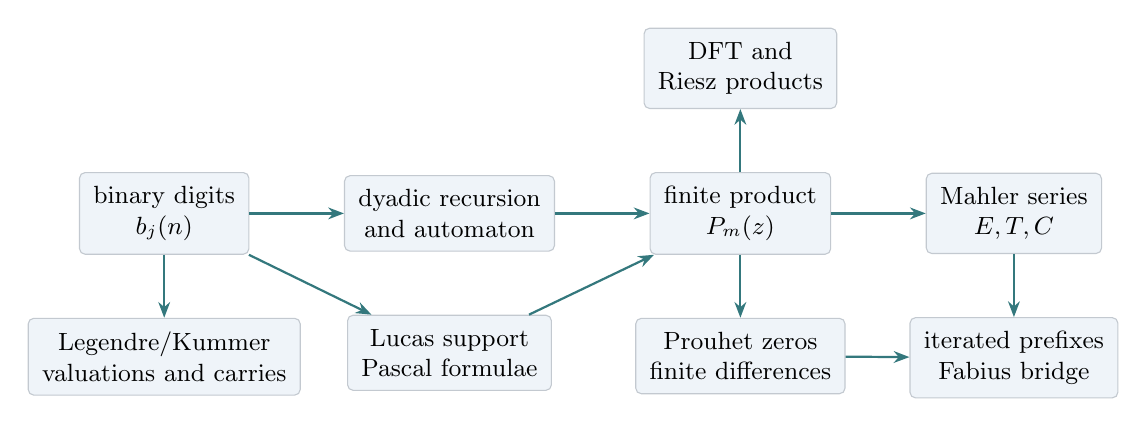
\begin{tikzpicture}[
 node distance=8mm and 12mm,
 every node/.style={draw=rulegray,rounded corners=2pt,fill=softblue,
                    align=center,inner sep=5pt,font=\small},
 arrow/.style={-{Stealth[length=2mm]},thick,draw=softteal}]
 \node (digits) {binary digits\\$b_j(n)$};
 \node (rec) [right=of digits] {dyadic recursion\\and automaton};
 \node (prod) [right=of rec] {finite product\\$P_m(z)$};
 \node (prouhet) [below=of prod] {Prouhet zeros\\finite differences};
 \node (fourier) [above=of prod] {DFT and\\Riesz products};
 \node (val) [below=of digits] {Legendre/Kummer\\valuations and carries};
 \node (pascal) [below=of rec] {Lucas support\\Pascal formulae};
 \node (mahler) [right=of prod] {Mahler series\\$E,T,C$};
 \node (fabius) [below=of mahler] {iterated prefixes\\Fabius bridge};
 \draw[arrow] (digits)--(rec);
 \draw[arrow] (rec)--(prod);
 \draw[arrow] (digits)--(val);
 \draw[arrow] (digits)--(pascal);
 \draw[arrow] (pascal)--(prod);
 \draw[arrow] (prod)--(prouhet);
 \draw[arrow] (prod)--(fourier);
 \draw[arrow] (prod)--(mahler);
 \draw[arrow] (prouhet)--(fabius);
 \draw[arrow] (mahler)--(fabius);
\end{tikzpicture}
\end{center}

\section{Formalization roadmap for \texttt{ProveIt}}

\subsection{Already central in the existing development}

The repository already contains Lean developments around the
binomial--logarithm formula, finite generating products, prefix sums, and the
Fabius bridge.  The consolidated article suggests organizing further work by
mathematical dependency rather than by the order in which formulae were
discovered.

\subsection{Layer 1: binary and finite algebra}

A foundational module should contain:
\begin{itemize}
 \item the recursions $\eps_{2n}=\eps_n$ and $\eps_{2n+1}=-\eps_n$;
 \item block multiplicativity $\eps_{2^ma+b}=\eps_a\eps_b$;
 \item the XOR character law;
 \item the finite coefficient product $P_m(z)$ over a general commutative ring;
 \item reciprocity and the cyclotomic factorization of $P_m$.
\end{itemize}
These statements need only finite sums, finite products, and bit lemmas.

\subsection{Layer 2: valuations and Pascal support}

The next layer depends on base-two digit-sum identities:
\begin{itemize}
 \item Legendre's formula $\vtwo(n!)=n-\bitsum(n)$;
 \item $\vtwo\binom{2n}{n}=\bitsum(n)$;
 \item Kummer's carry formula and the carry-corrected sign law;
 \item Lucas's submask criterion and the Glaisher count;
 \item the modulo-three log-free formula;
 \item odd multinomial support $r^{\bitsum(n)}$.
\end{itemize}
For formalization, it is preferable to state equalities in $\N$ before taking
parity in $\mathbb Z/2\mathbb Z$.

\subsection{Layer 3: polynomials, moments, and finite differences}

This layer should prove:
\begin{itemize}
 \item the order-$m$ zero of $P_m$ at $1$;
 \item Prouhet cancellation for powers and falling factorials;
 \item the operator identity with mixed finite differences;
 \item the exact cubature formula by iterated fundamental theorem of calculus;
 \item the all-moment composition formula;
 \item sparse submask Prouhet identities.
\end{itemize}
A reusable abstraction would take arbitrary steps $h_0,\ldots,h_{m-1}$ and
weights from $\prod_j(1-z^{h_j})$, with Thue--Morse as the dyadic instance.

\subsection{Layer 4: formal power series}

The formal series layer should include:
\begin{itemize}
 \item $E(z)=(1-z)E(z^2)$ and the coefficient recurrence from its logarithmic
       derivative;
 \item the Bell-polynomial and Hessenberg determinant formulae;
 \item the characteristic-two quadratic equation for $\Theta$;
 \item the integer algebraic lift and its coefficientwise parity theorem;
 \item the iterated-prefix generating series $E(z)/(1-z)^k$;
 \item the autocorrelation functional equation, once existence and recursion
       of $\eta$ are available.
\end{itemize}
The finite-product versions should be proved first; analytic convergence can
then be added as a separate wrapper.

\subsection{Layer 5: Fourier and analysis}

The final layer contains:
\begin{itemize}
 \item root-of-unity evaluation and the exact DFT sine product;
 \item the modulo-three rarefaction theorem;
 \item normalized finite Riesz products and their Fourier coefficients;
 \item Mellin and Dirichlet integral representations;
 \item finite reciprocal-power positivity and logarithmic-product inequalities;
 \item the Fabius/up-function limits already developed elsewhere in the
       repository.
\end{itemize}
Gelfond's sharp estimate, singular continuity, transcendence, and irrationality
measure should initially enter as cited external theorems rather than targets
for immediate re-formalization.

\subsection{Suggested module graph}

\begin{lstlisting}[style=pseudo,caption={Possible Lean module decomposition}]
ThueMorse.Basic
  -> ThueMorse.Blocks
  -> ThueMorse.BooleanCharacter
  -> ThueMorse.FiniteProduct

ThueMorse.DigitSum
  -> ThueMorse.Valuation
  -> ThueMorse.Carries
  -> ThueMorse.Pascal
  -> ThueMorse.Multinomial

ThueMorse.FiniteProduct
  -> ThueMorse.Prouhet
  -> ThueMorse.FiniteDifference
  -> ThueMorse.Moments
  -> ThueMorse.SparseProuhet
  -> ThueMorse.DFT
  -> ThueMorse.RarefactionMod3

ThueMorse.FormalSeries
  -> ThueMorse.Mahler
  -> ThueMorse.RulerRecurrence
  -> ThueMorse.BellDeterminant
  -> ThueMorse.CharTwo
  -> ThueMorse.IntegerLift
  -> ThueMorse.IteratedPrefix

ThueMorse.Autocorrelation
  -> ThueMorse.RieszProduct
  -> ThueMorse.AutocorrelationGenerating
\end{lstlisting}

\section{Conclusions}

The four drafts become considerably clearer when organized around one finite
product.  Binary digits give its coefficient signs; Lucas turns the same binary
support into Pascal's odd positions; Kummer measures the carry obstruction to
multiplicativity; the zero at $1$ gives Prouhet cancellation and exact finite
differences; unit-circle evaluation gives ordinary Fourier transforms; squared
moduli give Riesz products; division by powers of $1-z$ gives iterated prefix
sums; and passage to the infinite product gives Mahler equations and analytic
constants.

The most useful new consequences of the consolidation are not isolated
formulae but bridges.  The modulo-three rarefied sums show that cubic-root
Fourier extremizers have exact arithmetic-progression meaning.  The functional
equation for the autocorrelation series shows that the spectral coefficients
belong to the same Mahler universe as the original sequence.  The
characteristic-two quadratic and the characteristic-zero natural boundary
show how strongly the ambient field changes the algebraic nature of an
automatic series.  Finally, the sparse Pascal-support identities reveal that
every binary row index carries its own Prouhet system, with cancellation order
exactly equal to its digit sum.

The resulting atlas is therefore more than a catalogue.  It is a dependency
network in which the sequence's arithmetic, combinatorial, harmonic, and
analytic appearances can be translated into one another by short exact
arguments.

\appendix

\section{The first sixty-four values}

The zero--one word, grouped into blocks of sixteen, is
\begin{align*}
 0\text{--}15:&\quad 0110100110010110,\\
16\text{--}31:&\quad 1001011001101001,\\
32\text{--}47:&\quad 1001011001101001,\\
48\text{--}63:&\quad 0110100110010110.
\end{align*}
The corresponding signed blocks are
\begin{align*}
 0\text{--}15:&\quad +--+-++--++-+--+,\\
16\text{--}31:&\quad -++-+--++--+-++-,\\
32\text{--}47:&\quad -++-+--++--+-++-,\\
48\text{--}63:&\quad +--+-++--++-+--+.
\end{align*}
The repeated middle blocks and reversed signs at dyadic boundaries are direct
instances of \cref{eq:block-recursion,eq:reflection-rule}.

\section{Identity crosswalk}

\begin{longtable}{>{\raggedright\arraybackslash}p{0.27\textwidth}
                  >{\raggedright\arraybackslash}p{0.31\textwidth}
                  >{\raggedright\arraybackslash}p{0.31\textwidth}}
\toprule
Target & Exact formula & Main bridge \\
\midrule
\endhead
Individual sign & $\eps_n=(-1)^{\bitsum(n)}$ & definition \\
Digit floors & $\bitsum(n)=n-\sum_{j\ge1}\lfloor n/2^j\rfloor$ & telescoping bit extraction \\
Factorial valuation & $\eps_n=(-1)^{n-\vtwo(n!)}$ & Legendre \\
Central binomial & $\eps_n=(-1)^{\vtwo\binom{2n}{n}}$ & Legendre plus shift invariance \\
Carries & $\eps_{a+b}=\eps_a\eps_b(-1)^{\vtwo\binom{a+b}{a}}$ & Kummer \\
Pascal support & $\mathcal O(n)=2^{\bitsum(n)}$ & Lucas \\
Log-free Pascal & $\tau(n)=[\mathcal O(n)]_3-1$ & powers of two modulo three \\
Multinomial support & $\mathcal O_r(n)=r^{\bitsum(n)}$ & carry-free digit allocation \\
Finite product & $P_m(z)=\prod_{j<m}(1-z^{2^j})$ & binary subset expansion \\
Prouhet & $\sum_{n<2^m}\eps_nn^r=0$ for $r<m$ & order-$m$ zero at $1$ \\
Finite differences & $\sum\eps_nf(x+n)=(-1)^m\prod_j\Delta_{2^j}f(x)$ & shift-operator factorization \\
DFT & $\widehat\eps_m(k)=P_m(\e^{-2\pi\ii k/2^m})$ & evaluation at roots of unity \\
Rarefaction mod $3$ & \cref{eq:mod3-even-block,eq:mod3-odd-block} & cubic-root filter \\
Riesz product & $2^{-m}|P_m(\e^{2\pi\ii x})|^2=\prod_j(1-\cos2\pi2^jx)$ & squared Fourier magnitude \\
Mahler series & $E(z)=(1-z)E(z^2)$ & least-significant-bit split \\
Autocorrelation series & $2zC(z)=1-(1-z)^2C(z^2)$ & even--odd correlation recursion \\
Characteristic two & $(1+z)^3\Theta^2+(1+z)^2\Theta+z=0$ & Frobenius $\Theta(z^2)=\Theta(z)^2$ \\
Iterated prefixes & $\sum S_n^{(k)}z^n=E(z)/(1-z)^k$ & discrete integration \\
\bottomrule
\end{longtable}

\section{Source-draft consolidation map}

\begin{longtable}{>{\raggedright\arraybackslash}p{0.18\textwidth}
                  >{\raggedright\arraybackslash}p{0.36\textwidth}
                  >{\raggedright\arraybackslash}p{0.36\textwidth}}
\toprule
Draft & Distinct emphasis retained here & Principal consolidated sections \\
\midrule
\endhead
Draft 1 & central-binomial valuation, carries, floor and Boolean formulae,
logarithmic derivative, Bell and determinant forms, analytic transforms &
Sections 2--4, 9--10, 18 \\
Draft 2 & master catalogue, higher dyadic moments, exact cubature, automata,
tensor/Walsh forms, DFT and computational organization &
Sections 2, 11--12, 15, 23 \\
Draft 3 & fractional-part formula, Catalan and multinomial support, sparse
Pascal Prouhet systems, characteristic-two algebraicity, autocorrelation and
Riesz products, base-$q$ extension &
Sections 3--6, 12, 16--17, 21 \\
Draft 4 & sinc sign encoding, evil/odious enumerators, log-free Pascal formula,
one-parameter row statistic, integer algebraic lift, infinite products, and
iterated-prefix/Fabius bridge &
Sections 3, 7--8, 10, 13, 19--20 \\
New consolidation & exact modulo-three rarefied sums, autocorrelation generating
equation, Gelfond-extremizer synthesis, natural-boundary contrast, integrated
formalization graph &
Sections 14, 16, 22, 24 \\
\bottomrule
\end{longtable}

\begin{thebibliography}{99}

\bibitem{alloucheshallit2003}
J.-P. Allouche and J. Shallit,
\emph{Automatic Sequences: Theory, Applications, Generalizations},
Cambridge University Press, 2003.

\bibitem{alloucheshallitUbiquitous}
J.-P. Allouche and J. Shallit,
The ubiquitous Prouhet--Thue--Morse sequence,
in \emph{Sequences and Their Applications}, Springer, 1999, pp.~1--16.

\bibitem{alloucheriasatshallit2019}
J.-P. Allouche, S. Riasat, and J. Shallit,
More infinite products: Thue--Morse and the gamma function,
\emph{The Ramanujan Journal} \textbf{49}(1) (2019), 115--128,
DOI \nolinkurl{10.1007/s11139-017-9981-7}.

\bibitem{apww1998}
J.-P. Allouche, J. Peyri\`ere, Z.-X. Wen, and Z.-Y. Wen,
Hankel determinants of the Thue--Morse sequence,
\emph{Annales de l'Institut Fourier} \textbf{48} (1998), 1--27.

\bibitem{baakegrimm2008}
M. Baake and U. Grimm,
The singular continuous diffraction measure of the Thue--Morse chain,
\emph{Journal of Physics A: Mathematical and Theoretical}
\textbf{41} (2008), 422001.

\bibitem{bugeaud2011}
Y. Bugeaud,
On the rational approximation to the Thue--Morse--Mahler numbers,
\emph{Annales de l'Institut Fourier} \textbf{61} (2011), 2065--2076,
DOI \nolinkurl{10.5802/aif.2666}.

\bibitem{bugeaudhan2014}
Y. Bugeaud and G.-N. Han,
A combinatorial proof of the non-vanishing of Hankel determinants of the
Thue--Morse sequence,
\emph{Electronic Journal of Combinatorics} \textbf{21}(3) (2014), Paper P3.26,
DOI \nolinkurl{10.37236/3831}.

\bibitem{christol1979}
G. Christol, T. Kamae, M. Mend\`es France, and G. Rauzy,
Suites alg\'ebriques, automates et substitutions,
\emph{Bulletin de la Soci\'et\'e Math\'ematique de France}
\textbf{108} (1980), 401--419.

\bibitem{carlson1921}
F. Carlson,
\"Uber Potenzreihen mit ganzzahligen Koeffizienten,
\emph{Mathematische Zeitschrift} \textbf{9} (1921), 1--13,
DOI \nolinkurl{10.1007/BF01378331}.

\bibitem{gelfond1968}
A. O. Gelfond,
Sur les nombres qui ont des propri\'et\'es additives et multiplicatives donn\'ees,
\emph{Acta Arithmetica} \textbf{13} (1968), 259--265,
DOI \nolinkurl{10.4064/aa-13-3-259-265}.

\bibitem{mahler1929}
K. Mahler,
Arithmetische Eigenschaften der L\"osungen einer Klasse von
Funktionalgleichungen,
\emph{Mathematische Annalen} \textbf{101} (1929), 342--366.

\bibitem{queffelec2010}
M. Queff\'elec,
\emph{Substitution Dynamical Systems -- Spectral Analysis},
2nd ed., Lecture Notes in Mathematics 1294, Springer, 2010.

\bibitem{queffelec2018}
M. Queff\'elec,
Questions around the Thue--Morse sequence,
\emph{Uniform Distribution Theory} \textbf{13}(1) (2018), 1--25,
DOI \nolinkurl{10.1515/udt-2018-0001}.

\bibitem{robbins1979}
D. P. Robbins,
Solution to Problem E2692,
\emph{American Mathematical Monthly} \textbf{86} (1979), 394--395.

\bibitem{thue1912}
A. Thue,
\"Uber die gegenseitige Lage gleicher Teile gewisser Zeichenreihen,
\emph{Norske Videnskabers Selskabs Skrifter, I. Mat.-Naturv. Klasse}
(1912), no.~1, 1--67.

\bibitem{woods1978}
D. R. Woods,
Elementary problem proposal E2692,
\emph{American Mathematical Monthly} \textbf{85} (1978), 48.

\end{thebibliography}

\end{document}
